% !TeX program = xelatex
% Biên dịch bằng XeLaTeX; latexmk tự cập nhật mục lục và trích dẫn.
% Trình bày theo Thesis Template for OU Students; nội dung các chương giữ nguyên.
\documentclass[oneside,a4paper,12pt]{extreport}
\usepackage{lmodern}
% extreport không hỗ trợ trực tiếp tùy chọn 13pt của template.
\usepackage[fontsize=13pt]{fontsize}
\usepackage{fontspec}
\setmainfont{Times New Roman}
\usepackage[top=35mm,bottom=20mm,left=35mm,right=20mm,footskip=15mm,includefoot]{geometry}
\usepackage{graphicx}
\usepackage{booktabs,tabularx,fvextra,xurl}
\graphicspath{{./}{report/}{../}}
\usepackage[unicode,hidelinks]{hyperref}
\usepackage{titlesec}
\titleformat{\chapter}[display]
    {\normalfont\bfseries\large}{\chaptername\ \thechapter}{10pt}{\huge}
\titlespacing*{\chapter}{0pt}{-10pt}{20pt}
\titleformat{\section}{\normalfont\bfseries\large}{\thesection}{1em}{}
\titleformat{\subsection}{\normalfont\bfseries\normalsize}{\thesubsection}{1em}{}
\usepackage{setspace}
\onehalfspacing
\usepackage{indentfirst}
\usepackage{tikz}
\usetikzlibrary{calc}
\renewcommand{\chaptername}{Chương}
\renewcommand{\figurename}{Hình}
\renewcommand{\tablename}{Bảng}
\renewcommand{\contentsname}{Mục lục}
\renewcommand{\listfigurename}{Danh sách hình}
\renewcommand{\listtablename}{Danh sách bảng}
\renewcommand{\appendixname}{Phụ lục}
\renewcommand{\bibname}{Tài liệu tham khảo}
\setlength{\parindent}{1cm}
\setlength{\parskip}{0pt}
\setlength{\emergencystretch}{2em}

% Điền thông tin thực tế tại đây; không dùng tên mẫu trong template gốc.
\newcommand{\danhSachSinhVien}{[Họ tên và MSSV các thành viên]}
\newcommand{\tenGiangVien}{[Tên giảng viên hướng dẫn]}
\newcommand{\tenDeTai}{NGHIÊN CỨU VÀ KIỂM THỬ\\BẢO MẬT REST API\\TRÊN OWASP crAPI}
\newcommand{\namBaoCao}{2026}
\newcommand{\khungBia}{%
    \begin{tikzpicture}[remember picture,overlay]
        \draw[line width=2pt]
        ($(current page.north west)+(3.5cm,-2cm)$)
        rectangle ($(current page.south east)+(-1.5cm,3cm)$);
    \end{tikzpicture}%
}

\hypersetup{pageanchor=false}
\begin{document}

\begin{titlepage}
    \thispagestyle{empty}
    \begin{center}
        BỘ GIÁO DỤC VÀ ĐÀO TẠO\\
        TRƯỜNG ĐẠI HỌC MỞ THÀNH PHỐ HỒ CHÍ MINH\\[1cm]
        
\includegraphics[width=3cm]{ou-logo.jpg}\\[1cm]
        \vspace{1.5cm}
        {\Large\bfseries \tenDeTai\par}
        \vspace{1.5cm}
        {\large BÁO CÁO BÀI TẬP LỚN\\
        MÔN AN TOÀN THÔNG TIN\par}
        \vfill
        TP. Hồ Chí Minh, \namBaoCao
    \end{center}
    \khungBia
\end{titlepage}

\begin{titlepage}
    \thispagestyle{empty}
    \begin{center}
        BỘ GIÁO DỤC VÀ ĐÀO TẠO\\
        TRƯỜNG ĐẠI HỌC MỞ THÀNH PHỐ HỒ CHÍ MINH\\[1cm]
        
\includegraphics[width=3cm]{ou-logo.jpg}\\[0.8cm]
        \danhSachSinhVien\par
        \vspace{1cm}
        {\Large\bfseries \tenDeTai\par}
        \vspace{1cm}
        {\large BÁO CÁO BÀI TẬP LỚN\\
        MÔN AN TOÀN THÔNG TIN\par}
        \vspace{1cm}
        Giảng viên hướng dẫn:\\
        \textbf{\tenGiangVien}
        \vfill
        TP. Hồ Chí Minh, \namBaoCao
    \end{center}
    \khungBia
\end{titlepage}

\pagenumbering{roman}
\hypersetup{pageanchor=true}
\phantomsection
\addcontentsline{toc}{chapter}{Mục lục}
\tableofcontents
\clearpage
\phantomsection
\addcontentsline{toc}{chapter}{Danh sách hình}
\listoffigures
\clearpage
\phantomsection
\addcontentsline{toc}{chapter}{Danh sách bảng}
\listoftables
\clearpage
\pagenumbering{arabic}

\chapter{Giới thiệu bài toán và hệ thống thực nghiệm}

\section{Giới thiệu bài toán}

Trong các ứng dụng web, những thao tác quen thuộc như đăng nhập, xem thông
tin cá nhân, đặt hàng hay đăng bài thường được thực hiện thông qua API.
Có thể hiểu API là nơi tiếp nhận yêu cầu từ giao diện, xử lý nghiệp vụ và
trả lại kết quả. Với REST API, các yêu cầu thường được gửi qua HTTP, còn
dữ liệu trao đổi thường có dạng JSON.

Ví dụ, khi người dùng chọn xem thông tin một chiếc xe, trình duyệt gửi
yêu cầu đến API kèm thông tin xác thực và mã định danh của xe. Máy chủ
cần kiểm tra người gửi là ai, người đó có quyền xem chiếc xe này hay
không, rồi mới trả về những dữ liệu được phép cung cấp. Nếu chỉ kiểm tra
người dùng đã đăng nhập mà bỏ qua quyền sở hữu xe, API có thể làm lộ
thông tin của người khác.

Vấn đề đặt ra là: \textbf{hệ thống có kiểm tra đầy đủ danh tính, quyền
truy cập và dữ liệu đầu vào cho từng yêu cầu API hay không?} Việc giao
diện không hiển thị một nút chức năng hoặc một trường dữ liệu chưa đủ
để bảo đảm an toàn. Người dùng có thể gửi yêu cầu trực tiếp đến API,
thay đổi mã đối tượng hoặc bổ sung các thuộc tính mà giao diện không
cho nhập. Vì vậy, những quy tắc bảo mật cần được thực thi ở phía máy chủ.

Trong đề tài này, nhóm nghiên cứu và thực nghiệm các lỗ hổng REST API
trên OWASP crAPI. Mục tiêu là hiểu cách lỗ hổng xuất hiện, kiểm chứng tác
động bằng yêu cầu và phản hồi thực tế, từ đó đề xuất biện pháp khắc phục.
Các bài kiểm thử tự động được sử dụng để hỗ trợ kiểm tra lại hành vi
bảo mật và giúp người khác tái hiện kết quả.

\section{Giới thiệu hệ thống OWASP crAPI}

OWASP crAPI (Completely Ridiculous API) là ứng dụng được xây dựng có chủ
đích với các lỗ hổng để phục vụ học tập và thực hành bảo mật API~\cite{crapi}. Trong
đề tài, crAPI đóng vai trò hệ thống mục tiêu; nhóm triển khai và kiểm
thử hệ thống này trong môi trường cục bộ được phép.

Ứng dụng mô phỏng các hoạt động gắn với người dùng và phương tiện, cùng
các chức năng như quản lý tài khoản, tương tác cộng đồng và xử lý đơn
hàng. Những nghiệp vụ này tạo ra các tình huống cần kiểm soát quyền:
ai được xem thông tin xe, ai được thao tác trên nội dung, và ai được thay
đổi trạng thái của một giao dịch.

crAPI được tổ chức theo kiến trúc microservices, tức là chia hệ thống
thành nhiều dịch vụ phụ trách các nhóm chức năng khác nhau. Hình
\ref{fig:crapi-architecture} trình bày sơ đồ được sử dụng để giới thiệu
các thành phần và mối liên hệ tổng quan của hệ thống.

\begin{figure}[p]
    \centering
    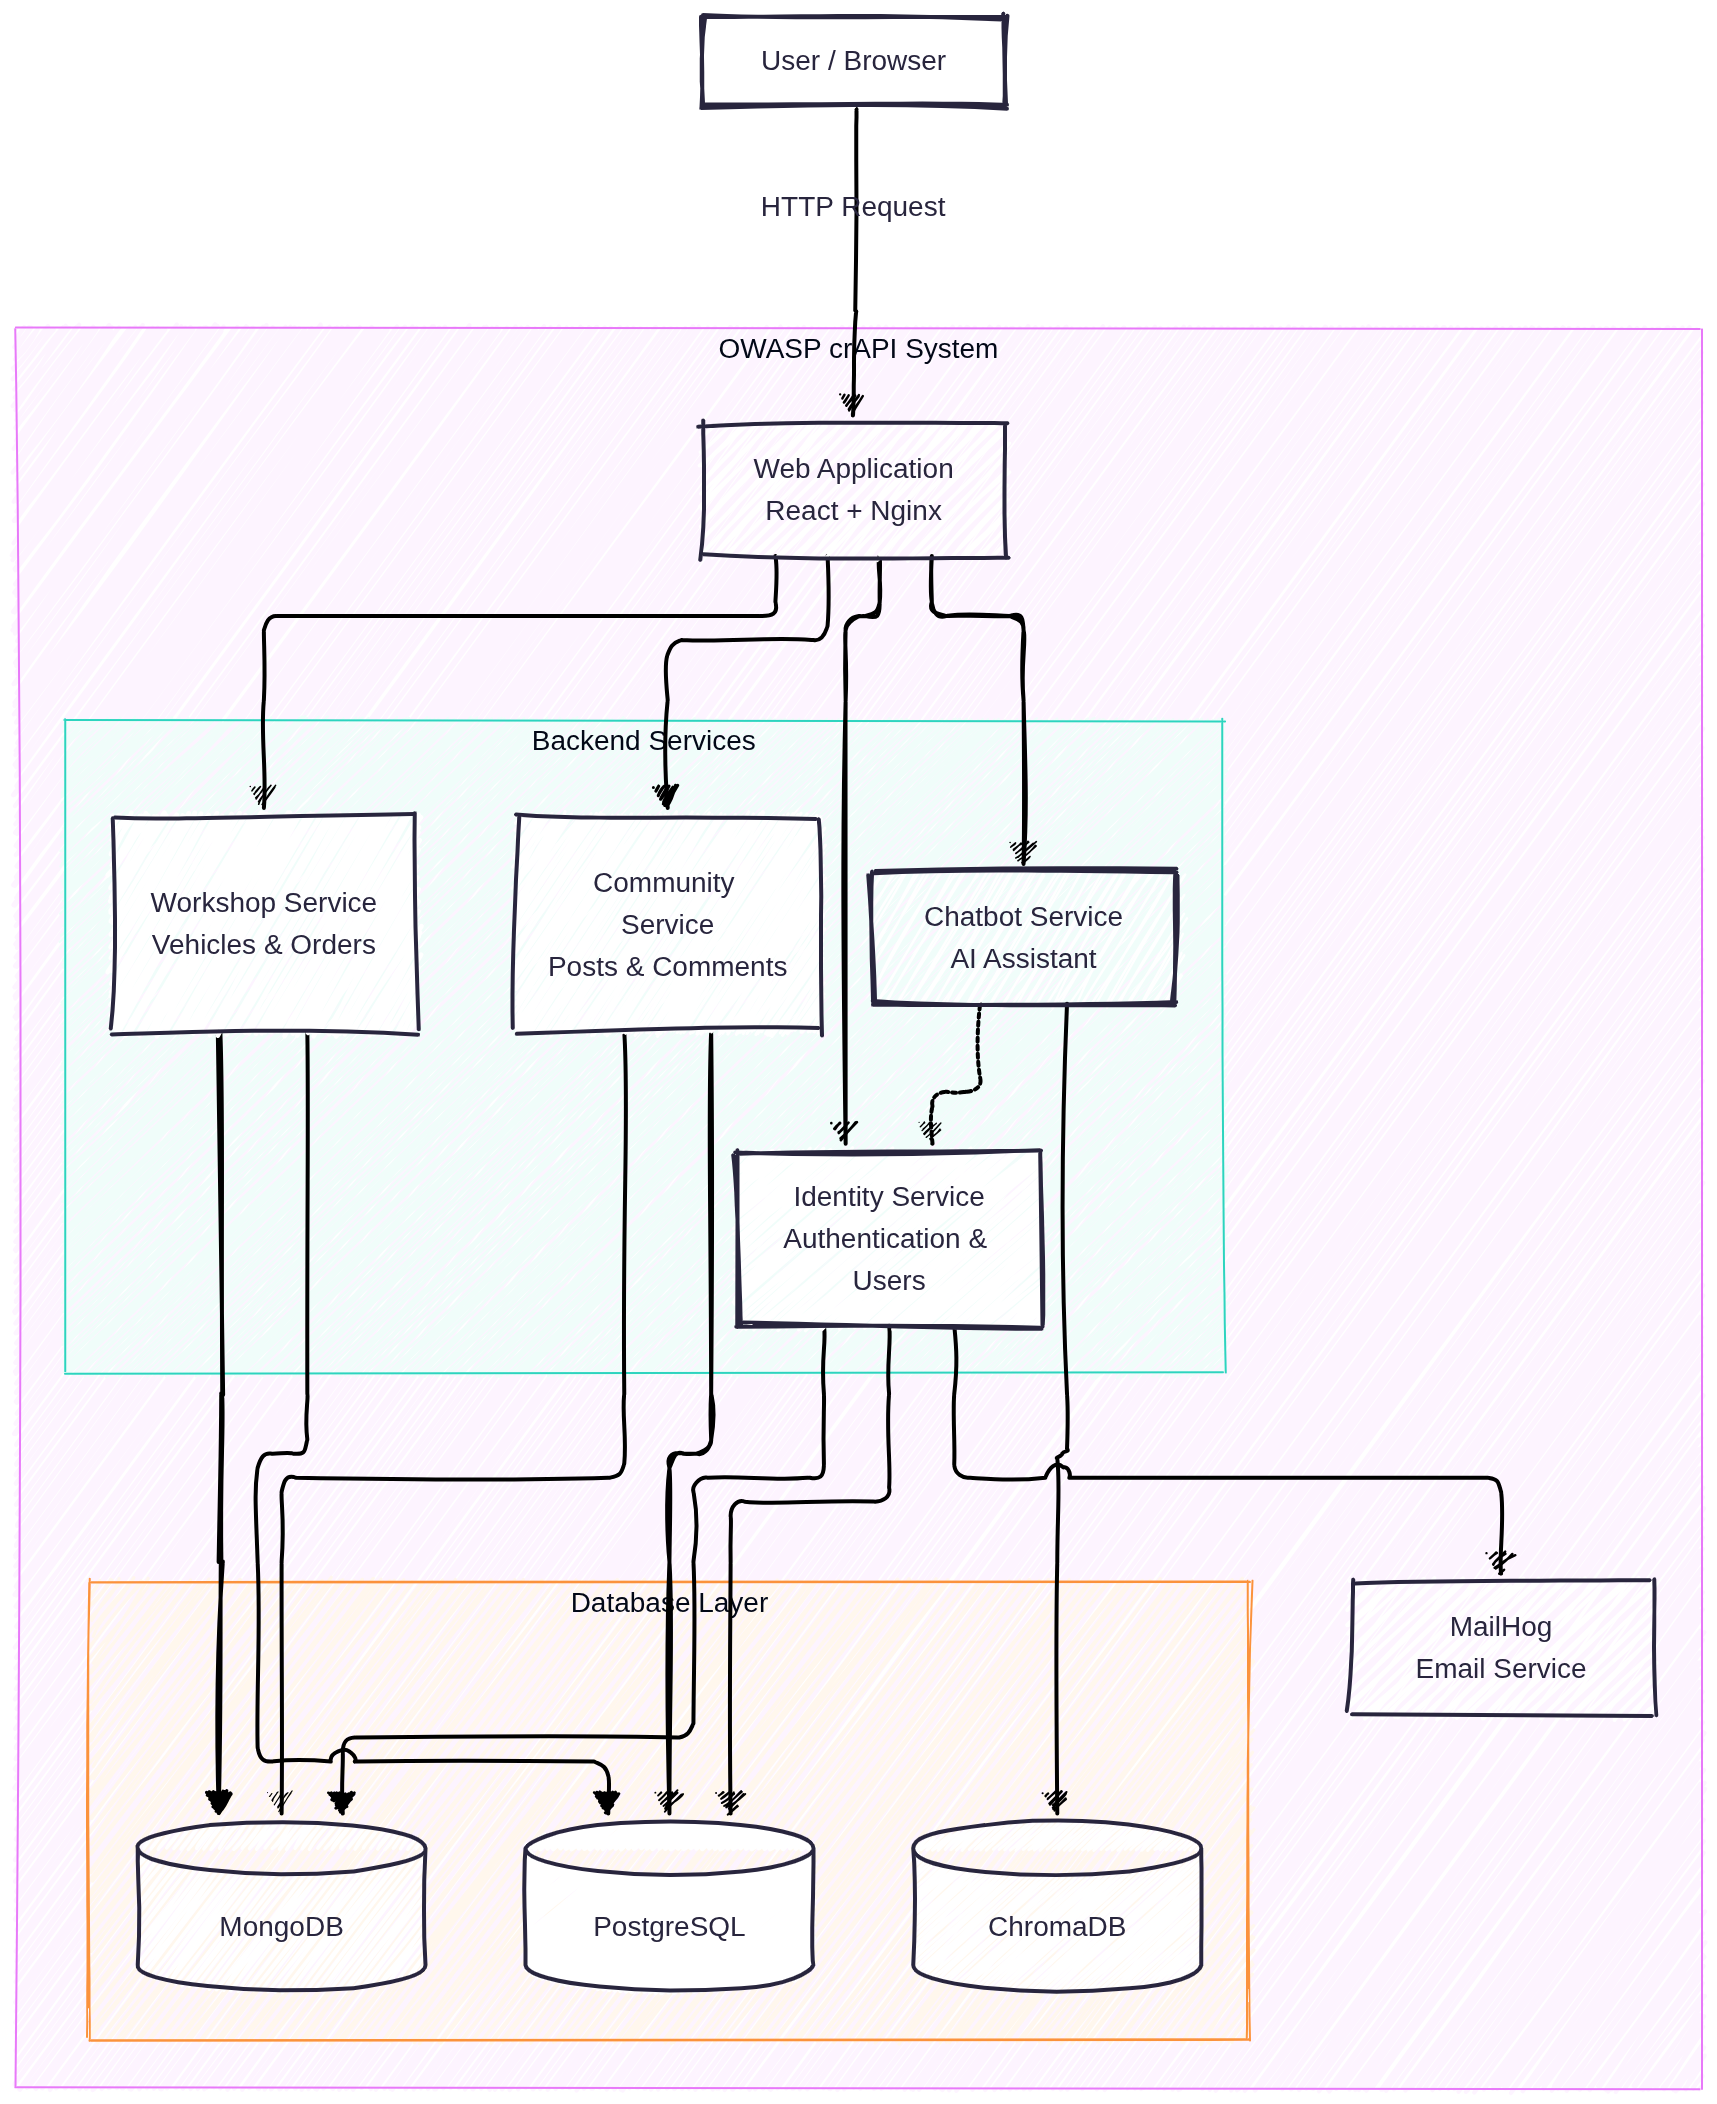
\includegraphics[width=\textwidth,height=0.83\textheight,keepaspectratio]{crapi-architecture.png}
    \caption{Sơ đồ tổng quan hệ thống OWASP crAPI (hình được cung cấp cho báo cáo).}
    \label{fig:crapi-architecture}
\end{figure}

\subsection{Giao diện và các dịch vụ xử lý}

Theo sơ đồ, người dùng truy cập ứng dụng qua trình duyệt. Thành phần
\textbf{Web Application} sử dụng React cho giao diện và Nginx để phục vụ
ứng dụng, chuyển tiếp các yêu cầu API đến dịch vụ phía sau. Các dịch vụ
được thể hiện trong sơ đồ gồm:

\begin{itemize}
    \item \textbf{Identity Service:} phụ trách xác thực và thông tin người
    dùng, liên quan đến việc xác định danh tính khi truy cập hệ thống.
    \item \textbf{Workshop Service:} xử lý các nghiệp vụ liên quan đến
    phương tiện và đơn hàng.
    \item \textbf{Community Service:} phục vụ các hoạt động cộng đồng như
    bài đăng và bình luận.
    \item \textbf{Chatbot Service:} cung cấp chức năng trợ lý AI theo
    kiến trúc được mô tả trong hình.
\end{itemize}

Việc tách thành các dịch vụ giúp phân chia trách nhiệm xử lý, nhưng cũng
đòi hỏi các yêu cầu bảo mật phải được thực hiện nhất quán. Một yêu cầu đã
đi qua giao diện hoặc có thông tin đăng nhập vẫn cần được kiểm tra quyền
tại chức năng xử lý tài nguyên tương ứng.

\subsection{Lưu trữ dữ liệu và dịch vụ thư thử nghiệm}

Lớp dữ liệu trong sơ đồ gồm \textbf{MongoDB}, \textbf{PostgreSQL} và
\textbf{ChromaDB}. Các dịch vụ backend đọc hoặc ghi dữ liệu thông qua
những thành phần lưu trữ này; ChromaDB được thể hiện là thành phần lưu
trữ phục vụ Chatbot Service. Người dùng thông thường tương tác với dữ
liệu thông qua API của ứng dụng.

\textbf{MailHog} là dịch vụ tiếp nhận và hiển thị email trong môi trường
thử nghiệm, hỗ trợ quan sát các luồng có gửi thư mà không cần gửi email
đến hộp thư thật.

Sơ đồ trên được dùng để giải thích kiến trúc tổng quan. Thành phần thực
tế có thể khác giữa các phiên bản crAPI; cấu hình triển khai và commit
được sử dụng cần được ghi nhận trong phần môi trường thực nghiệm. Sự
xuất hiện của một thành phần trong sơ đồ không đồng nghĩa thành phần đó
đã được nhóm kiểm thử hoặc đã được xác nhận có lỗ hổng.

\section{Phạm vi và hướng tiếp cận}

Nhóm tập trung vào năm tình huống kiểm thử sau:
\begin{enumerate}
    \item \textbf{BOLA:} kiểm tra khả năng truy cập thông tin phương tiện
    của người khác khi thay đổi mã đối tượng trong yêu cầu.
    \item \textbf{BFLA:} kiểm tra khả năng gọi chức năng xóa video vượt
    quá quyền được cấp.
    \item \textbf{Excessive Data Exposure:} kiểm tra API có trả về dữ
    liệu nhạy cảm hoặc dữ liệu người gọi không được phép nhận hay không.
    \item \textbf{Mass Assignment:} kiểm tra khả năng thay đổi thuộc
    tính không được phép để tác động đến quy trình hoàn tiền đơn hàng.
    \item \textbf{Unauthenticated Access:} kiểm tra khả năng truy cập
    chức năng cần bảo vệ khi chưa xác thực.
\end{enumerate}

Với mỗi tình huống, nhóm khảo sát hành vi bình thường, xác định yêu cầu
bảo mật cần có, sau đó thay đổi yêu cầu API có kiểm soát và đối chiếu
phản hồi. Kết luận phải dựa trên bằng chứng thực nghiệm, phân biệt rõ
hành vi đã xác minh với giả thuyết hoặc biện pháp mới được đề xuất.

Toàn bộ hoạt động chỉ thực hiện trên instance crAPI do nhóm triển khai
cục bộ. Báo cáo sử dụng tài khoản và dữ liệu thử nghiệm; các bằng chứng
cần được loại bỏ mật khẩu, token, cookie và thông tin cá nhân trước khi
chia sẻ. Đề tài không xem việc triển khai crAPI là xây dựng một ứng dụng
mới, mà tập trung vào phương pháp kiểm thử, phân tích và kiểm chứng bảo
mật của nhóm.

\clearpage
\chapter{Lab 01: Truy cập trái phép thông tin phương tiện (BOLA)}
\label{chap:lab01}

\section{Bài toán và mục tiêu kiểm thử}

Trong crAPI, mỗi tài khoản có thể gắn với một phương tiện và xem vị trí
của xe trên Dashboard. Dữ liệu này chỉ nên được cung cấp cho chủ xe.
Lab 01 kiểm tra xem một người đã đăng nhập có thể đọc thông tin xe của
người khác bằng cách thay mã xe trong yêu cầu API hay không.

Lỗ hổng được khảo sát là \textbf{Broken Object Level Authorization
(BOLA)}, tức là thiếu kiểm tra quyền truy cập trên từng đối tượng.
Trong tình huống này, đối tượng là phương tiện~\cite{owasp-bola}. Hệ thống cần kiểm tra
cả hai điều: người gửi đã đăng nhập và người đó có quyền xem xe được yêu
cầu. Chỉ kiểm tra đăng nhập là chưa đủ.

\section{Chuẩn bị và hành vi mong đợi}

Thực nghiệm sử dụng crAPI chạy cục bộ tại
\url{http://127.0.0.1:8888}, với hai tài khoản thử nghiệm:
\begin{itemize}
    \item \textbf{User A:} người thực hiện yêu cầu kiểm thử, có xe riêng.
    \item \textbf{User B:} chủ xe mục tiêu, có xe riêng và đăng một bài
    viết trên Community.
\end{itemize}

Chrome DevTools được dùng để quan sát yêu cầu và phản hồi;
\texttt{curl} được dùng để gửi yêu cầu đã thay đổi; Python và
\texttt{pytest} được dùng để kiểm thử tự động.

API lấy vị trí xe có dạng:
\begin{Verbatim}[breaklines=true,breakanywhere=true,fontsize=\small]
GET /identity/api/v2/vehicle/{vehicle_id}/location
\end{Verbatim}

Trong đó, \texttt{vehicle\_id} là mã định danh xe. Yêu cầu gửi kèm token,
tức mã xác thực của tài khoản đã đăng nhập. Nếu User A yêu cầu xem xe
của mình, API được phép trả về dữ liệu. Nếu User A yêu cầu xem xe của
User B, API phải từ chối, chẳng hạn bằng mã \texttt{403 Forbidden} hoặc
\texttt{404 Not Found}, và không trả dữ liệu của User B.

\section{Các bước kiểm thử và bằng chứng}

\subsection{Thu thập mã xe của User B}

Đăng nhập bằng User A, mở Community và quan sát phản hồi trong tab
Network của Chrome DevTools. API danh sách bài viết được gọi là:
\begin{Verbatim}[breaklines=true,breakanywhere=true,fontsize=\small]
GET /community/api/v2/community/posts/recent
\end{Verbatim}

Phản hồi chứa bài viết của User B. Trong thông tin tác giả
(\texttt{author}), trường \texttt{vehicleid} trả về mã xe của User B.
Như vậy, User A có thể biết mã xe mục tiêu ngay từ bảng tin, không cần
đoán mã hoặc đăng nhập vào tài khoản User B.

\begin{figure}[htbp]
    \centering
    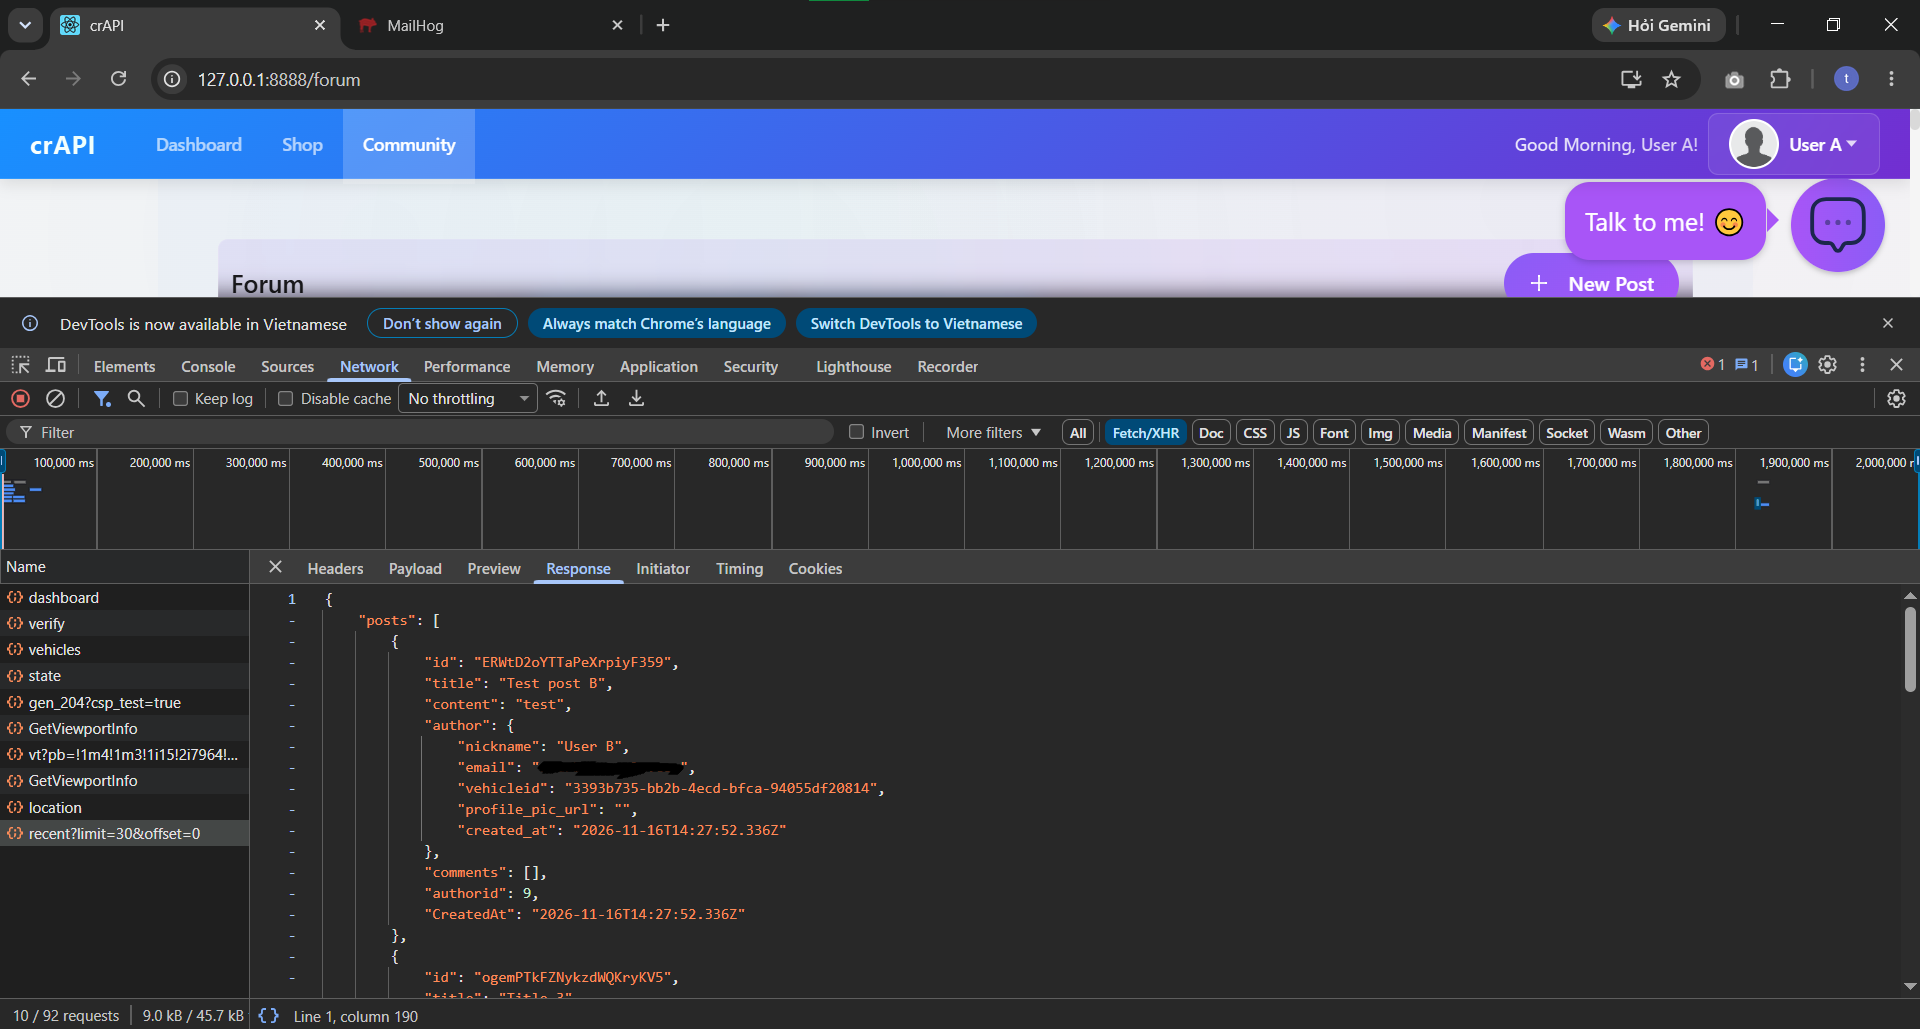
\includegraphics[width=\textwidth,height=0.55\textheight,keepaspectratio]{lab01/01-community-vehicleid-exposure.png}
    \caption{User A xem được mã xe của User B trong phản hồi API Community.}
    \label{fig:bola-vehicle-id}
\end{figure}

\subsection{Dùng phiên User A để yêu cầu vị trí xe của User B}

Giữ nguyên token của User A, nhưng đặt mã xe của User B vào đường dẫn
API lấy vị trí. Yêu cầu kiểm thử được ghi nhận như sau; token đã được
ẩn trước khi đưa vào báo cáo:

\begin{Verbatim}[breaklines=true,breakanywhere=true,fontsize=\small]
GET /identity/api/v2/vehicle/3393b735-bb2b-4ecd-bfca-94055df20814/location HTTP/1.1
Host: 127.0.0.1:8888
Authorization: Bearer <REDACTED_TOKEN_USER_A>
\end{Verbatim}

Điểm cần kiểm tra là \textbf{người gửi là User A, còn xe được yêu cầu
thuộc User B}. Việc biết mã xe không có nghĩa là User A được quyền xem
thông tin xe đó.

\subsection{Quan sát phản hồi}

Máy chủ không từ chối yêu cầu mà trả về \texttt{HTTP 200} cùng dữ liệu
của xe User B:

\begin{Verbatim}[breaklines=true,breakanywhere=true,fontsize=\small]
{
  "carId": "3393b735-bb2b-4ecd-bfca-94055df20814",
  "vehicleLocation": {
    "id": 2,
    "latitude": "31.284788",
    "longitude": "-92.471176"
  },
  "fullName": "User B",
  "email": "<REDACTED_EMAIL>"
}
\end{Verbatim}

\begin{figure}[htbp]
    \centering
    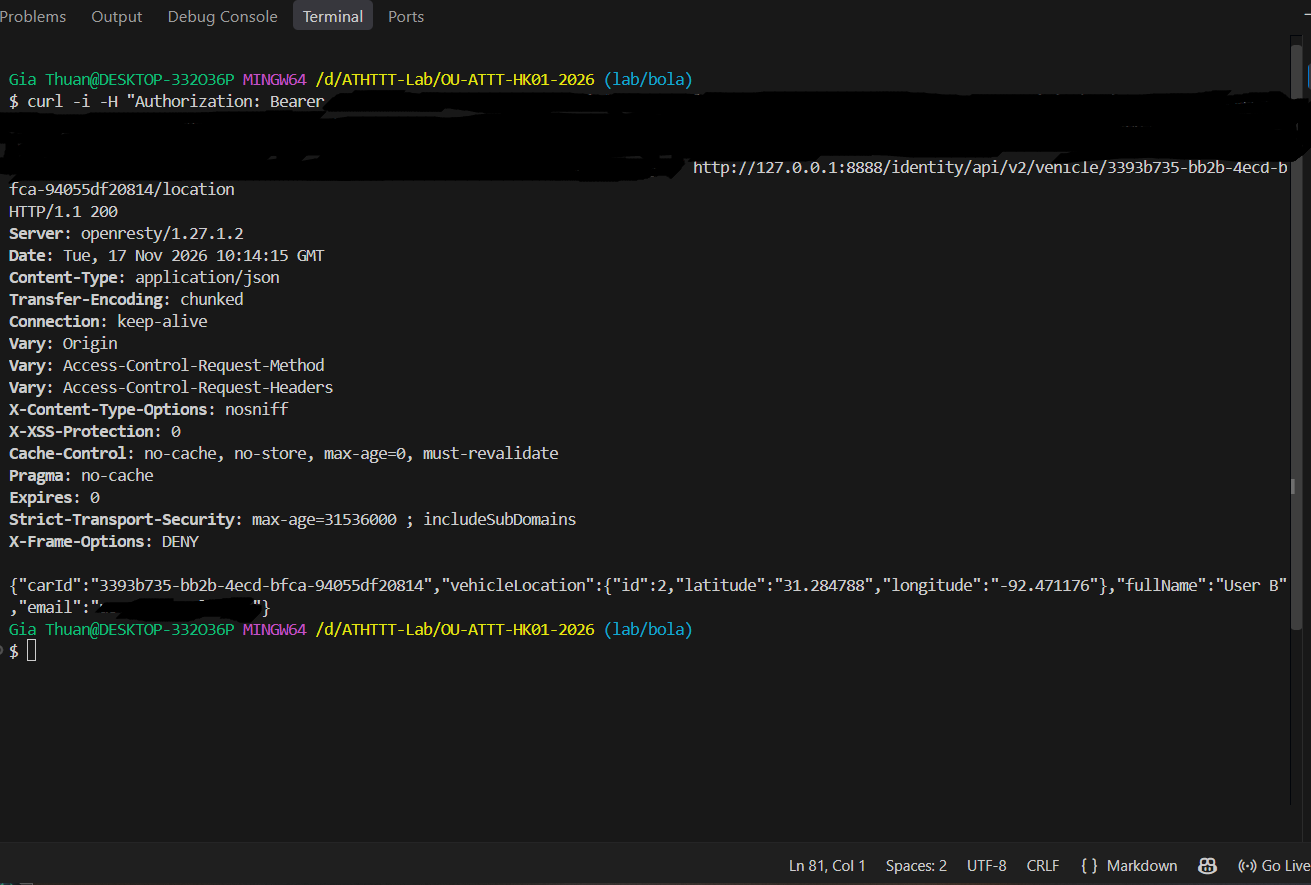
\includegraphics[width=\textwidth,height=0.55\textheight,keepaspectratio]{lab01/02-bola-unauthorized-vehicle-read.png}
    \caption{API trả về HTTP 200 và dữ liệu xe User B khi nhận yêu cầu từ User A.}
    \label{fig:bola-response}
\end{figure}

Kết quả này cho thấy User A đọc được tọa độ vị trí, tên và email gắn với
xe của User B. Đây là hành vi truy cập trái phép ở mức đối tượng, xác
nhận lỗi BOLA trong cặp tài khoản được kiểm thử. Lỗi đã được kiểm chứng
ở thao tác đọc; chưa có bằng chứng về khả năng sửa, xóa hoặc điều khiển xe.

\section{Kiểm thử tự động}

Bài kiểm thử nằm tại \path{tests/security/test_bola.py}.
Sau khi crAPI hoạt động và hai tài khoản đã có xe, chạy:

\begin{Verbatim}[breaklines=true,breakanywhere=true,fontsize=\small]
pytest tests/security/test_bola.py -v
\end{Verbatim}

Test đăng nhập hai tài khoản, lấy mã xe bằng phiên User B, rồi dùng
token của User A để yêu cầu vị trí xe đó. Việc lấy mã bằng phiên User B
là bước chuẩn bị dữ liệu cho test; bước thu thập mã qua Community được
kiểm chứng riêng ở phần thủ công.

Test yêu cầu API từ chối truy cập chéo với một trong các mã
\texttt{401}, \texttt{403}, \texttt{404}. Ảnh kết quả cho thấy test
\textbf{FAILED} vì nhận \texttt{200} cùng dữ liệu xe User B:

\begin{Verbatim}[breaklines=true,breakanywhere=true,fontsize=\small]
assert unauthorized_resp.status_code in {401, 403, 404}
E assert 200 in {401, 403, 404}
\end{Verbatim}

\begin{figure}[htbp]
    \centering
    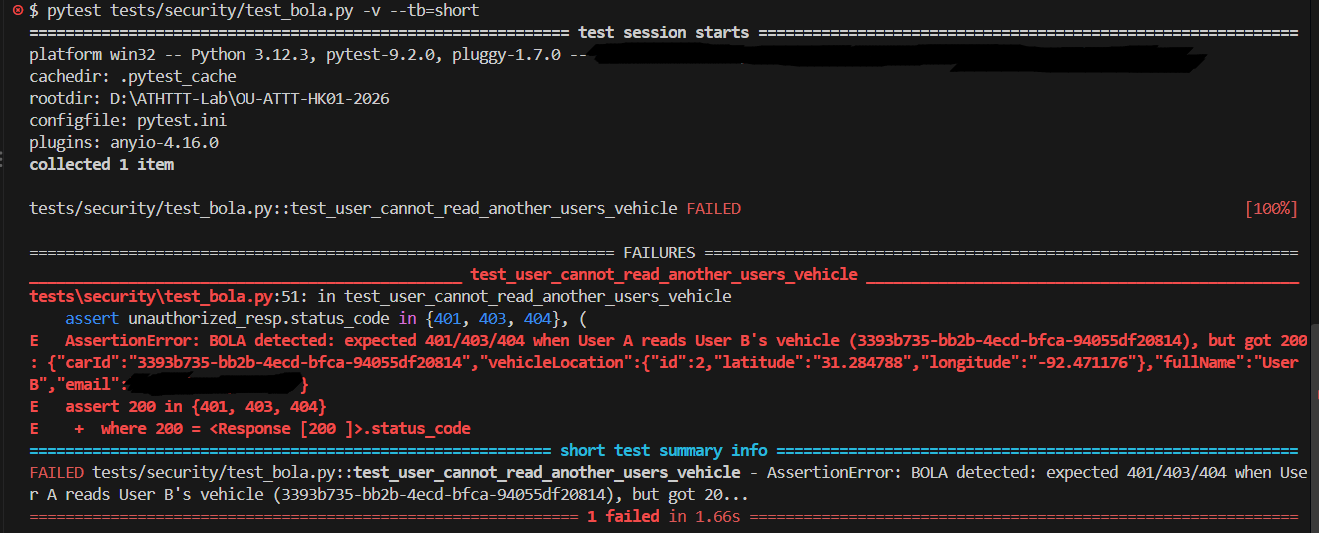
\includegraphics[width=\textwidth,height=0.42\textheight,keepaspectratio]{lab01/03-pytest-bola-failed.png}
    \caption{Test thất bại vì API cho phép đọc dữ liệu xe của tài khoản khác.}
    \label{fig:bola-test}
\end{figure}

Ở đây, test thất bại vì hành vi của API vi phạm yêu cầu bảo mật.
Lỗi đăng nhập hoặc thiếu dữ liệu thử nghiệm cũng có thể khiến test
thất bại, nhưng không phải bằng chứng BOLA. Ngược lại, test PASS chỉ
cho biết yêu cầu chéo bị từ chối theo điều kiện hiện có; cần kiểm tra
thêm quyền truy cập chính chủ trước khi kết luận bản vá đạt yêu cầu.

\section{Nguyên nhân và tác động}

Đối chiếu mã nguồn cho thấy hàm lấy vị trí xe tìm bản ghi theo mã xe,
lấy thông tin chủ xe rồi tạo phản hồi. Luồng xử lý này không đối chiếu
chủ xe với tài khoản đang gửi yêu cầu~\cite{crapi-vehicle}. Vì vậy, User A có token hợp lệ
vẫn nhận được dữ liệu của User B khi cung cấp đúng mã xe.

Việc API Community trả về \texttt{vehicleid} giúp User A tìm được mục
tiêu dễ hơn. Tuy nhiên, nguyên nhân chính vẫn là thiếu kiểm tra quyền
ở API lấy vị trí. Dù mã xe khó đoán hoặc bị ẩn khỏi bảng tin, API vẫn
phải từ chối người không có quyền.

Trong thực nghiệm, dữ liệu bị đọc trái phép gồm tọa độ vị trí, tên và
email của chủ xe. Với một hệ thống thực tế, việc lộ những thông tin này
có thể ảnh hưởng đến quyền riêng tư của người sử dụng.

\section{Biện pháp khắc phục và kết luận}

Biện pháp khắc phục được đề xuất gồm:
\begin{enumerate}
    \item Lấy danh tính người gọi từ phiên đã xác thực và kiểm tra quyền
    trên xe trước khi trả dữ liệu. Truy vấn cần ràng buộc cả mã xe và
    chủ sở hữu, thay vì chỉ dựa vào mã xe.
    \item Từ chối yêu cầu không có quyền bằng \texttt{403} hoặc
    \texttt{404}; phản hồi không chứa thông tin xe hay chủ xe.
    \item Loại bỏ \texttt{vehicleid} khỏi phản hồi Community nếu chức
    năng bảng tin không cần trường này. Đây là biện pháp giảm dữ liệu
    lộ ra, không thay thế việc kiểm tra quyền.
\end{enumerate}

Sau khi sửa, cần kiểm tra User A vẫn xem được xe của mình nhưng không
xem được xe User B, đồng thời User B vẫn truy cập được xe của mình.
Token không hợp lệ phải bị từ chối ở bước xác thực; không nên xem lỗi
xác thực là bằng chứng đã sửa đúng phân quyền.

Lab 01 ghi nhận API trả dữ liệu xe User B cho phiên User A. Kết quả
thủ công và ảnh chạy test cùng cho thấy lỗi BOLA ở chức năng lấy vị trí
xe. Các biện pháp trên mới là đề xuất; chưa có kết quả kiểm thử sau vá.


\clearpage
\chapter{Lab 02: Tài khoản thường gọi được chức năng quản trị (BFLA)}
\label{chap:lab02}

\section{Bài toán và mục tiêu kiểm thử}

Một tài khoản thông thường có thể quản lý nội dung của mình, nhưng
không được sử dụng chức năng quản trị để xóa video của người khác.
Lab này kiểm tra liệu máy chủ có ngăn tài khoản thường gọi API xóa
video dành cho quản trị viên hay không.

Lỗi được khảo sát là \textbf{Broken Function Level Authorization
(BFLA)}, tức thiếu kiểm soát quyền thực hiện chức năng, thuộc
API5:2023~\cite{owasp-bfla}. Khác với Lab 01 tập trung vào quyền trên
một tài nguyên, Lab 02 kiểm tra quyền sử dụng chức năng đặc quyền.
Không thể chỉ dựa vào tên đường dẫn có chữ \texttt{admin} để kết luận;
cần đối chiếu chức năng, quyền của người gọi và kết quả xử lý.

\section{Chuẩn bị và hành vi mong đợi}

crAPI chạy tại \url{http://127.0.0.1:8888}. Hai tài khoản thử nghiệm được
chuẩn bị với vai trò \texttt{ROLE\_USER}: \texttt{testerlab} thực hiện
yêu cầu kiểm thử, còn \texttt{ownerlab} sở hữu video mục tiêu có mã 6.

Theo báo cáo thực nghiệm, thao tác tải video ban đầu trả HTTP 404 nhưng
bản ghi vẫn được tạo trong cơ sở dữ liệu. Vì vậy, dữ liệu mục tiêu được
xác nhận bằng bản ghi video thay vì chỉ dựa vào phản hồi tải lên.

API cần kiểm tra là:
\begin{Verbatim}[breaklines=true,breakanywhere=true,fontsize=\small]
DELETE /identity/api/v2/admin/videos/{video_id}
\end{Verbatim}

Khi tài khoản thường gọi chức năng này, máy chủ phải trả
\texttt{403 Forbidden} và giữ nguyên video. Người đã đăng nhập không
đồng nghĩa với người có quyền quản trị.

\section{Các bước kiểm thử và bằng chứng}

\subsection{Gọi chức năng xóa bằng tài khoản thường}

Đăng nhập bằng \texttt{testerlab}, rồi dùng phiên đăng nhập đó gửi yêu
cầu xóa video của \texttt{ownerlab}:
\begin{Verbatim}[breaklines=true,breakanywhere=true,fontsize=\small]
DELETE /identity/api/v2/admin/videos/6 HTTP/1.1
Host: 127.0.0.1:8888
Authorization: Bearer <REDACTED>
\end{Verbatim}

Ảnh DevTools ghi nhận phản hồi \texttt{HTTP 200}. Giá trị
\texttt{ok: true} trong ảnh là thuộc tính của đối tượng phản hồi Fetch,
cho biết HTTP thành công; không phải bằng chứng riêng rằng dữ liệu đã
bị xóa. Vì vậy, cần kiểm tra thêm trạng thái video sau yêu cầu.


\begin{figure}[htbp]
    \centering
    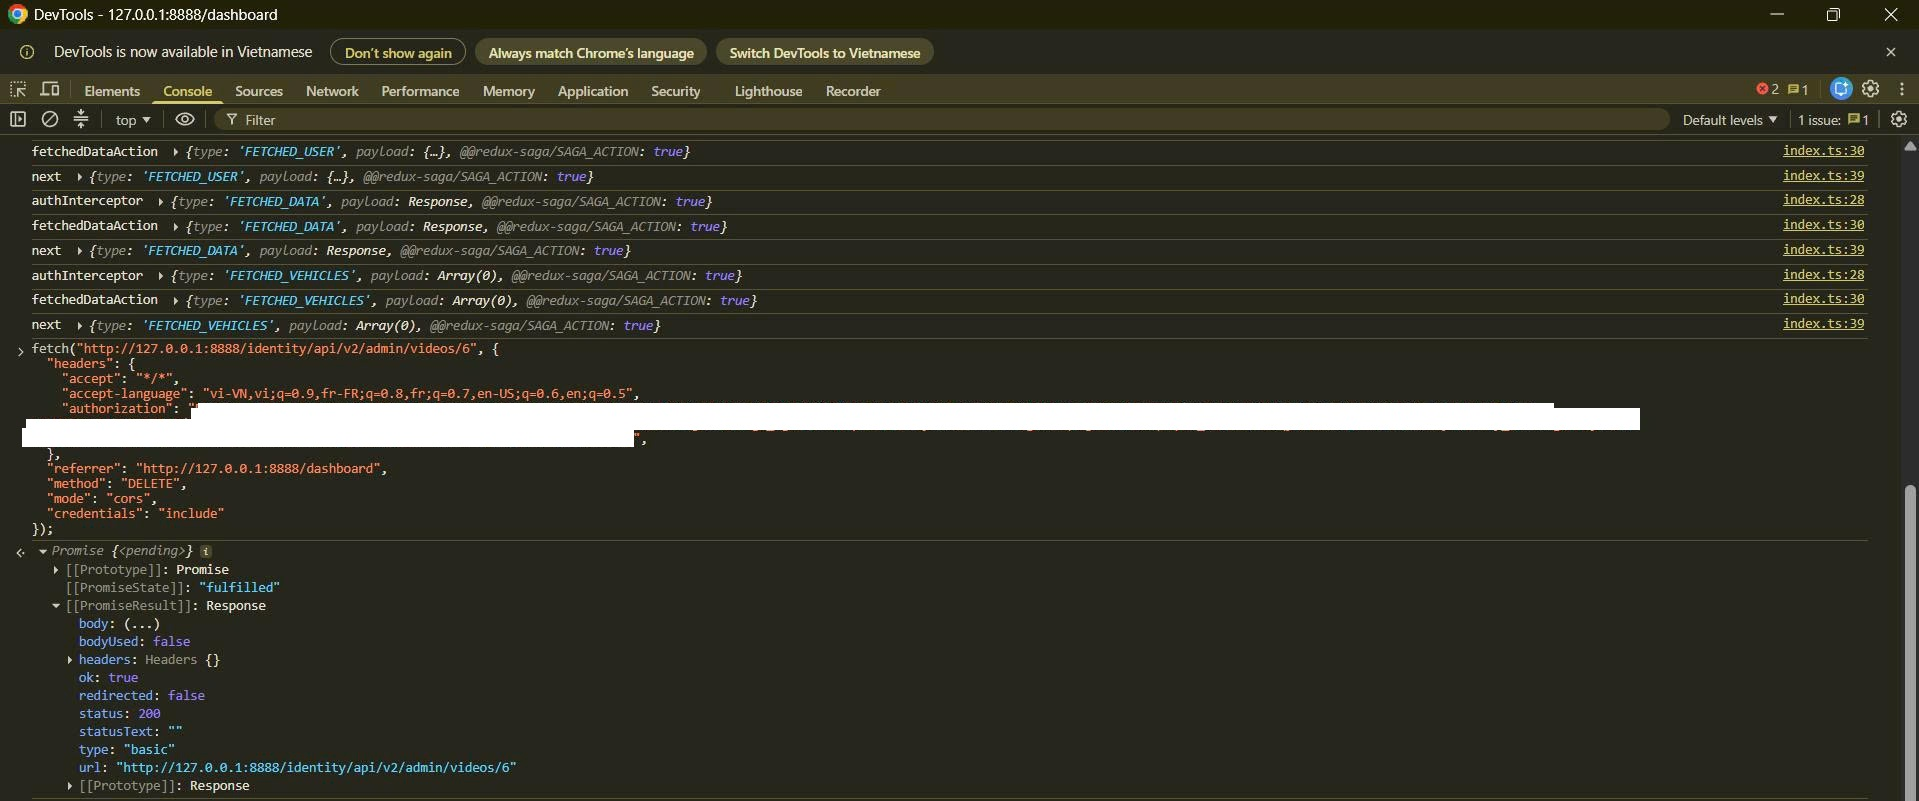
\includegraphics[width=\textwidth,height=0.65\textheight,keepaspectratio]{labs/02-bfla/evidence/bfla-devtools-delete-video.jpg}
    \caption{Tài khoản thường gửi DELETE đến chức năng quản trị và nhận HTTP 200.}
    \label{fig:lab2-delete}
\end{figure}


\subsection{Kiểm tra dữ liệu sau khi xóa}

Truy vấn cơ sở dữ liệu nối tài khoản chủ video với bảng video hồ sơ.
Kết quả vẫn có tài khoản \texttt{ownerlab}, nhưng các cột mã video và
tên video để trống. Kết hợp với dữ liệu mục tiêu đã chuẩn bị, kết quả
cho thấy video không còn gắn với hồ sơ chủ sở hữu sau yêu cầu DELETE.


\begin{figure}[htbp]
    \centering
    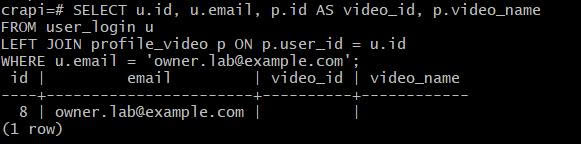
\includegraphics[width=\textwidth,height=0.65\textheight,keepaspectratio]{labs/02-bfla/evidence/bfla-verify-video-deleted.jpg}
    \caption{Sau yêu cầu xóa, truy vấn không còn tìm thấy video gắn với hồ sơ chủ sở hữu.}
    \label{fig:lab2-verify}
\end{figure}


Theo chuỗi thực nghiệm được ghi nhận, tài khoản thường đã gọi thành
công chức năng quản trị và tác động đến video của tài khoản khác.
Kết luận chỉ áp dụng cho chức năng xóa video được khảo sát, không suy
rộng thành quyền truy cập mọi chức năng quản trị.

\clearpage
\section{Nguyên nhân và biện pháp khắc phục}

Đối chiếu mã nguồn crAPI cho thấy controller chuyển mã video vào hàm
xử lý xóa. Hàm này lấy thông tin người gọi từ token, tìm video theo mã
rồi xóa, nhưng không kiểm tra vai trò quản trị trước khi thực hiện.
Đây là điểm thiếu kiểm soát quyền ở phía máy chủ.

Biện pháp khắc phục là yêu cầu vai trò ADMIN cho API xóa video, ở lớp
cấu hình bảo mật hoặc kiểm tra quyền tại phương thức xử lý. Quy tắc
phải khớp đường dẫn thực tế mà dịch vụ nhận được và được áp dụng trước
khi thay đổi dữ liệu. Khi tài khoản đã đăng nhập nhưng không đủ quyền,
API cần trả \texttt{403}.

Báo cáo thành viên ghi nhận đã bổ sung quy tắc yêu cầu ADMIN, cấu hình
phản hồi từ chối và triển khai lại dịch vụ Identity. Kết quả kiểm thử
lại được lưu trong \path{labs/02-bfla/evidence/bfla-retest.txt}.

\section{Kiểm thử tự động và kết luận}

File \path{tests/security/test_bfla.py} đăng nhập tài khoản thường rồi
gửi DELETE với mã video 999999 và yêu cầu nhận đúng \texttt{403}.
Test dùng mã không tồn tại để tránh xóa dữ liệu thật trong Lab. Cần
cấu hình tài khoản qua các biến môi trường trước khi chạy:
\begin{Verbatim}[breaklines=true,breakanywhere=true,fontsize=\small]
pytest -q tests/security/test_bfla.py -s
\end{Verbatim}

Log retest được bàn giao ghi:
\begin{Verbatim}[breaklines=true,breakanywhere=true,fontsize=\small]
1 passed in 0.84s
\end{Verbatim}

Kết quả này xác nhận yêu cầu từ tài khoản thường đã bị từ chối theo
điều kiện của test trong lần chạy sau sửa được báo cáo. Vì test dùng
mã không tồn tại, cần kiểm tra thêm trên một video thử có thật: USER
bị từ chối và video còn nguyên, còn ADMIN vẫn xóa được khi có quyền.
Log PASS hiện có chưa bao phủ hai điều kiện đó.

Lab ghi nhận lỗi BFLA ở chức năng xóa video và một kết quả retest sau
khi bổ sung phân quyền. Việc ẩn nút quản trị trên giao diện không thay
thế kiểm tra quyền tại API.

\clearpage
\chapter{Lab 03: API trả về dữ liệu không cần thiết (Excessive Data Exposure)}
\label{chap:lab03}

\section{Bài toán và mục tiêu kiểm thử}

Bảng tin cần nội dung bài viết và tên hiển thị của tác giả, nhưng không
nhất thiết cần email hoặc mã xe của người đó. Nếu máy chủ vẫn gửi những
trường này về trình duyệt, người dùng có thể đọc chúng trong phản hồi
API dù giao diện không hiển thị.

Đây là tình huống \textbf{Excessive Data Exposure}, tức API trả về dữ
liệu nhạy cảm nhiều hơn mức chức năng cần dùng. OWASP gọi nhóm lỗi này
là API3:2019~\cite{owasp-exposure}. Trong phiên bản 2023, quyền đọc từng
thuộc tính được xét trong nhóm Broken Object Property Level
Authorization~\cite{owasp-property}.

Lab khảo sát bảy API, đối chiếu dữ liệu trả về với nhu cầu của từng
chức năng. Một trường xuất hiện trong JSON là điểm cần đánh giá, không
tự động chứng minh mọi trường hợp đều là lỗ hổng nghiêm trọng.

\section{Chuẩn bị và cách kiểm thử}

crAPI chạy tại \url{http://127.0.0.1:8888}. Firefox được cấu hình đi qua
Burp Proxy ở cổng 8081 để quan sát lưu lượng. Cổng 8081 là cổng proxy,
không phải địa chỉ triển khai ứng dụng.

Người thực hiện đăng nhập tài khoản thử nghiệm, thao tác trên các chức
năng thợ sửa xe, Community, ảnh đại diện và phương tiện. Với mỗi thao
tác, gửi yêu cầu sang Burp Repeater rồi đối chiếu phản hồi JSON với
thông tin cần hiển thị. Các yêu cầu trong hồ sơ có thông tin xác thực;
Lab này không kết luận các API truy cập được khi chưa đăng nhập.

\section{Kết quả khảo sát và bằng chứng}

\subsection{Danh sách thợ sửa xe}
\begin{Verbatim}[breaklines=true,breakanywhere=true,fontsize=\small]
GET /workshop/api/mechanic/
\end{Verbatim}

Phản hồi chứa mã thợ sửa xe và đối tượng \texttt{user} gồm
\texttt{email}, \texttt{number}. Hai email được ghi nhận là
\texttt{jhon@example.com} và \texttt{james@example.com}; trường
\texttt{number} đang rỗng. Bằng chứng xác nhận API trả email, chưa chứng
minh số điện thoại bị lộ. Cần xác định email có phải thông tin liên hệ
được phép công khai của chức năng này hay không.


\begin{figure}[htbp]
    \centering
    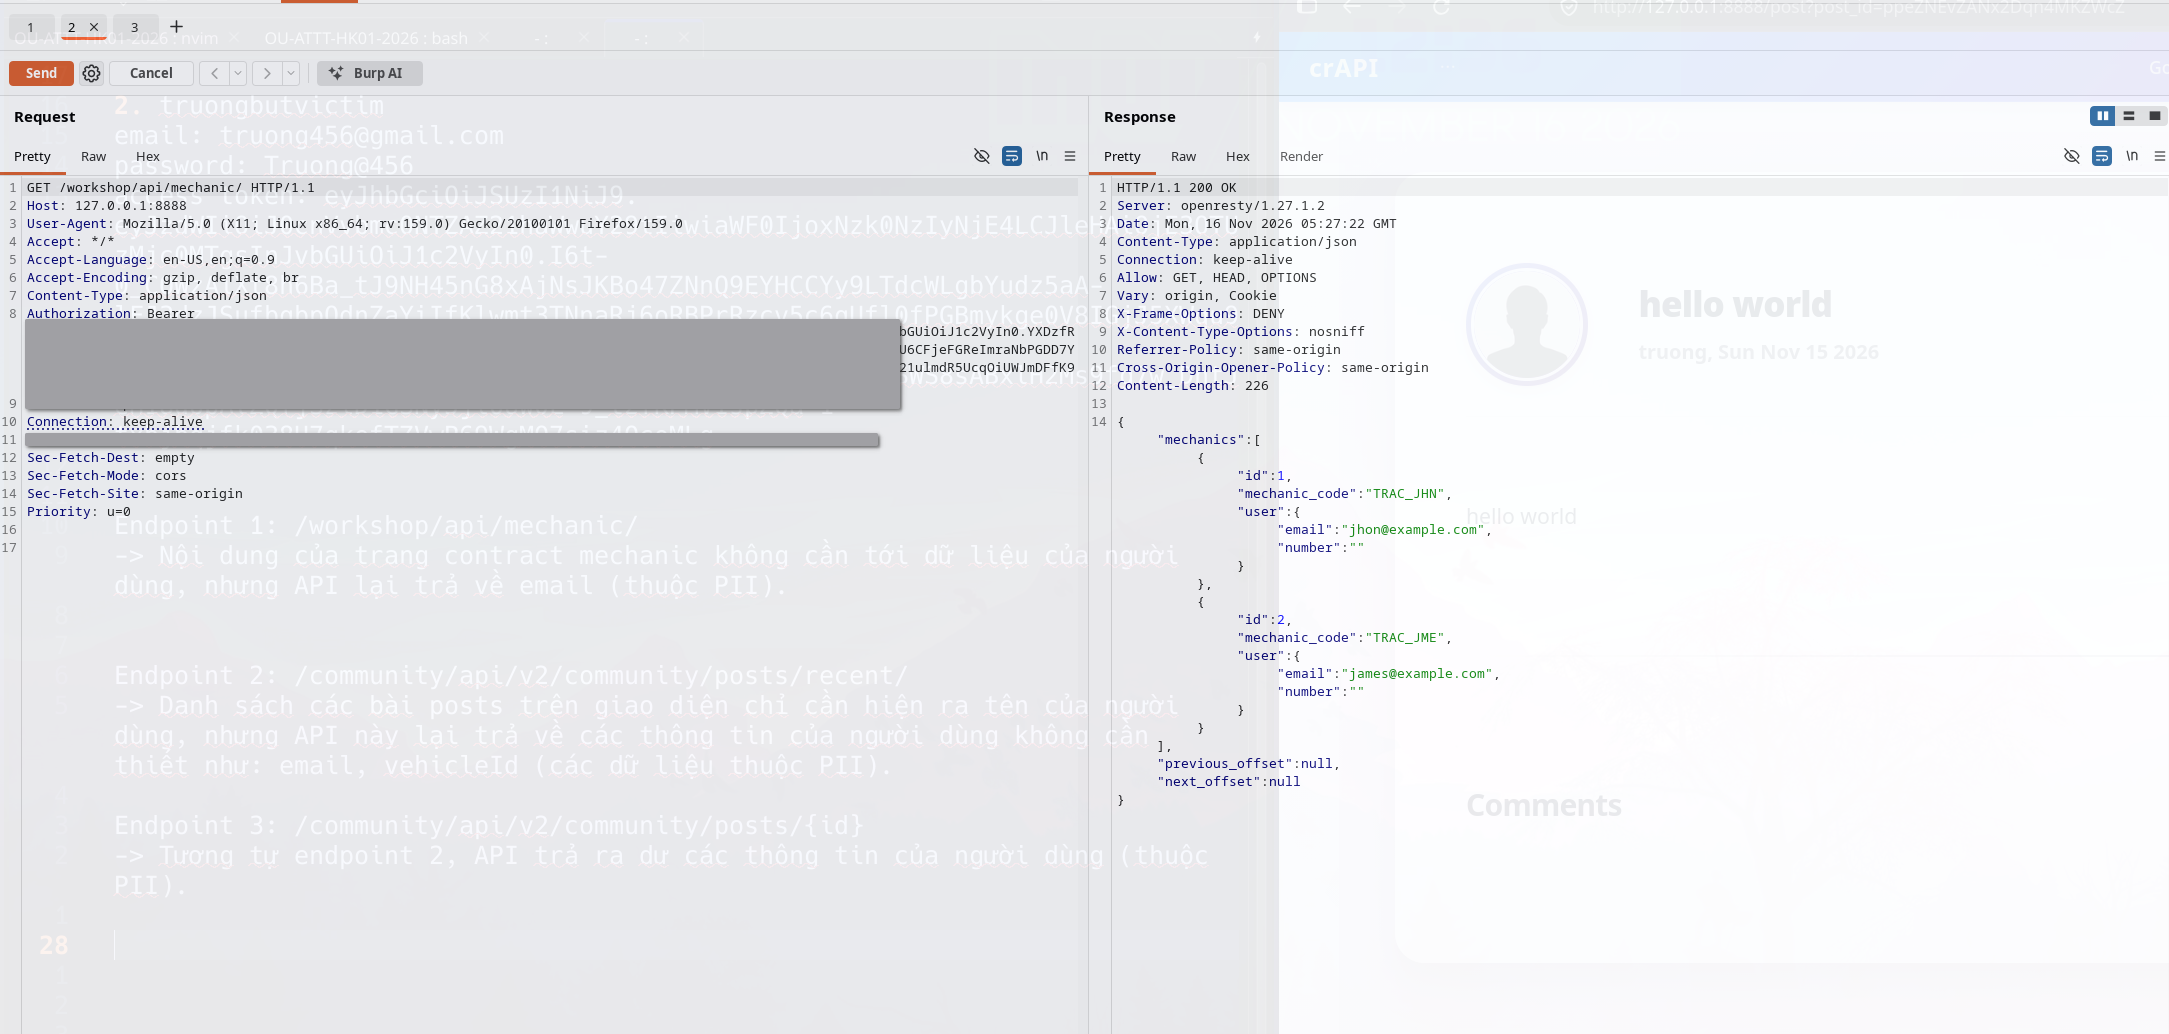
\includegraphics[width=\textwidth,height=0.52\textheight,keepaspectratio]{labs/03-data-exposure/evidence/endpoint-01-mechanic/mechanic.png}
    \caption{API thợ sửa xe trả email trong đối tượng user.}
    \label{fig:exposure-mechanic}
\end{figure}


\subsection{Danh sách và chi tiết bài viết}
\begin{Verbatim}[breaklines=true,breakanywhere=true,fontsize=\small]
GET /community/api/v2/community/posts/recent
GET /community/api/v2/community/posts/{id}
\end{Verbatim}

Danh sách bài viết chứa \texttt{email} và \texttt{vehicleid} của tác
giả, bao gồm cả tài khoản khác người đang đăng nhập. Phản hồi chi tiết
bài viết cũng chứa hai trường này. Mã xe không phục vụ trực tiếp cho
việc hiển thị nội dung bài viết, nhưng có thể trở thành đầu vào kiểm
thử quyền truy cập xe như trong Lab 01.

Trong các phản hồi đã lưu của hai API này, danh sách
\texttt{comments} đang rỗng; chưa có dữ liệu người bình luận để kết
luận tại hai yêu cầu đó.


\begin{figure}[htbp]
    \centering
    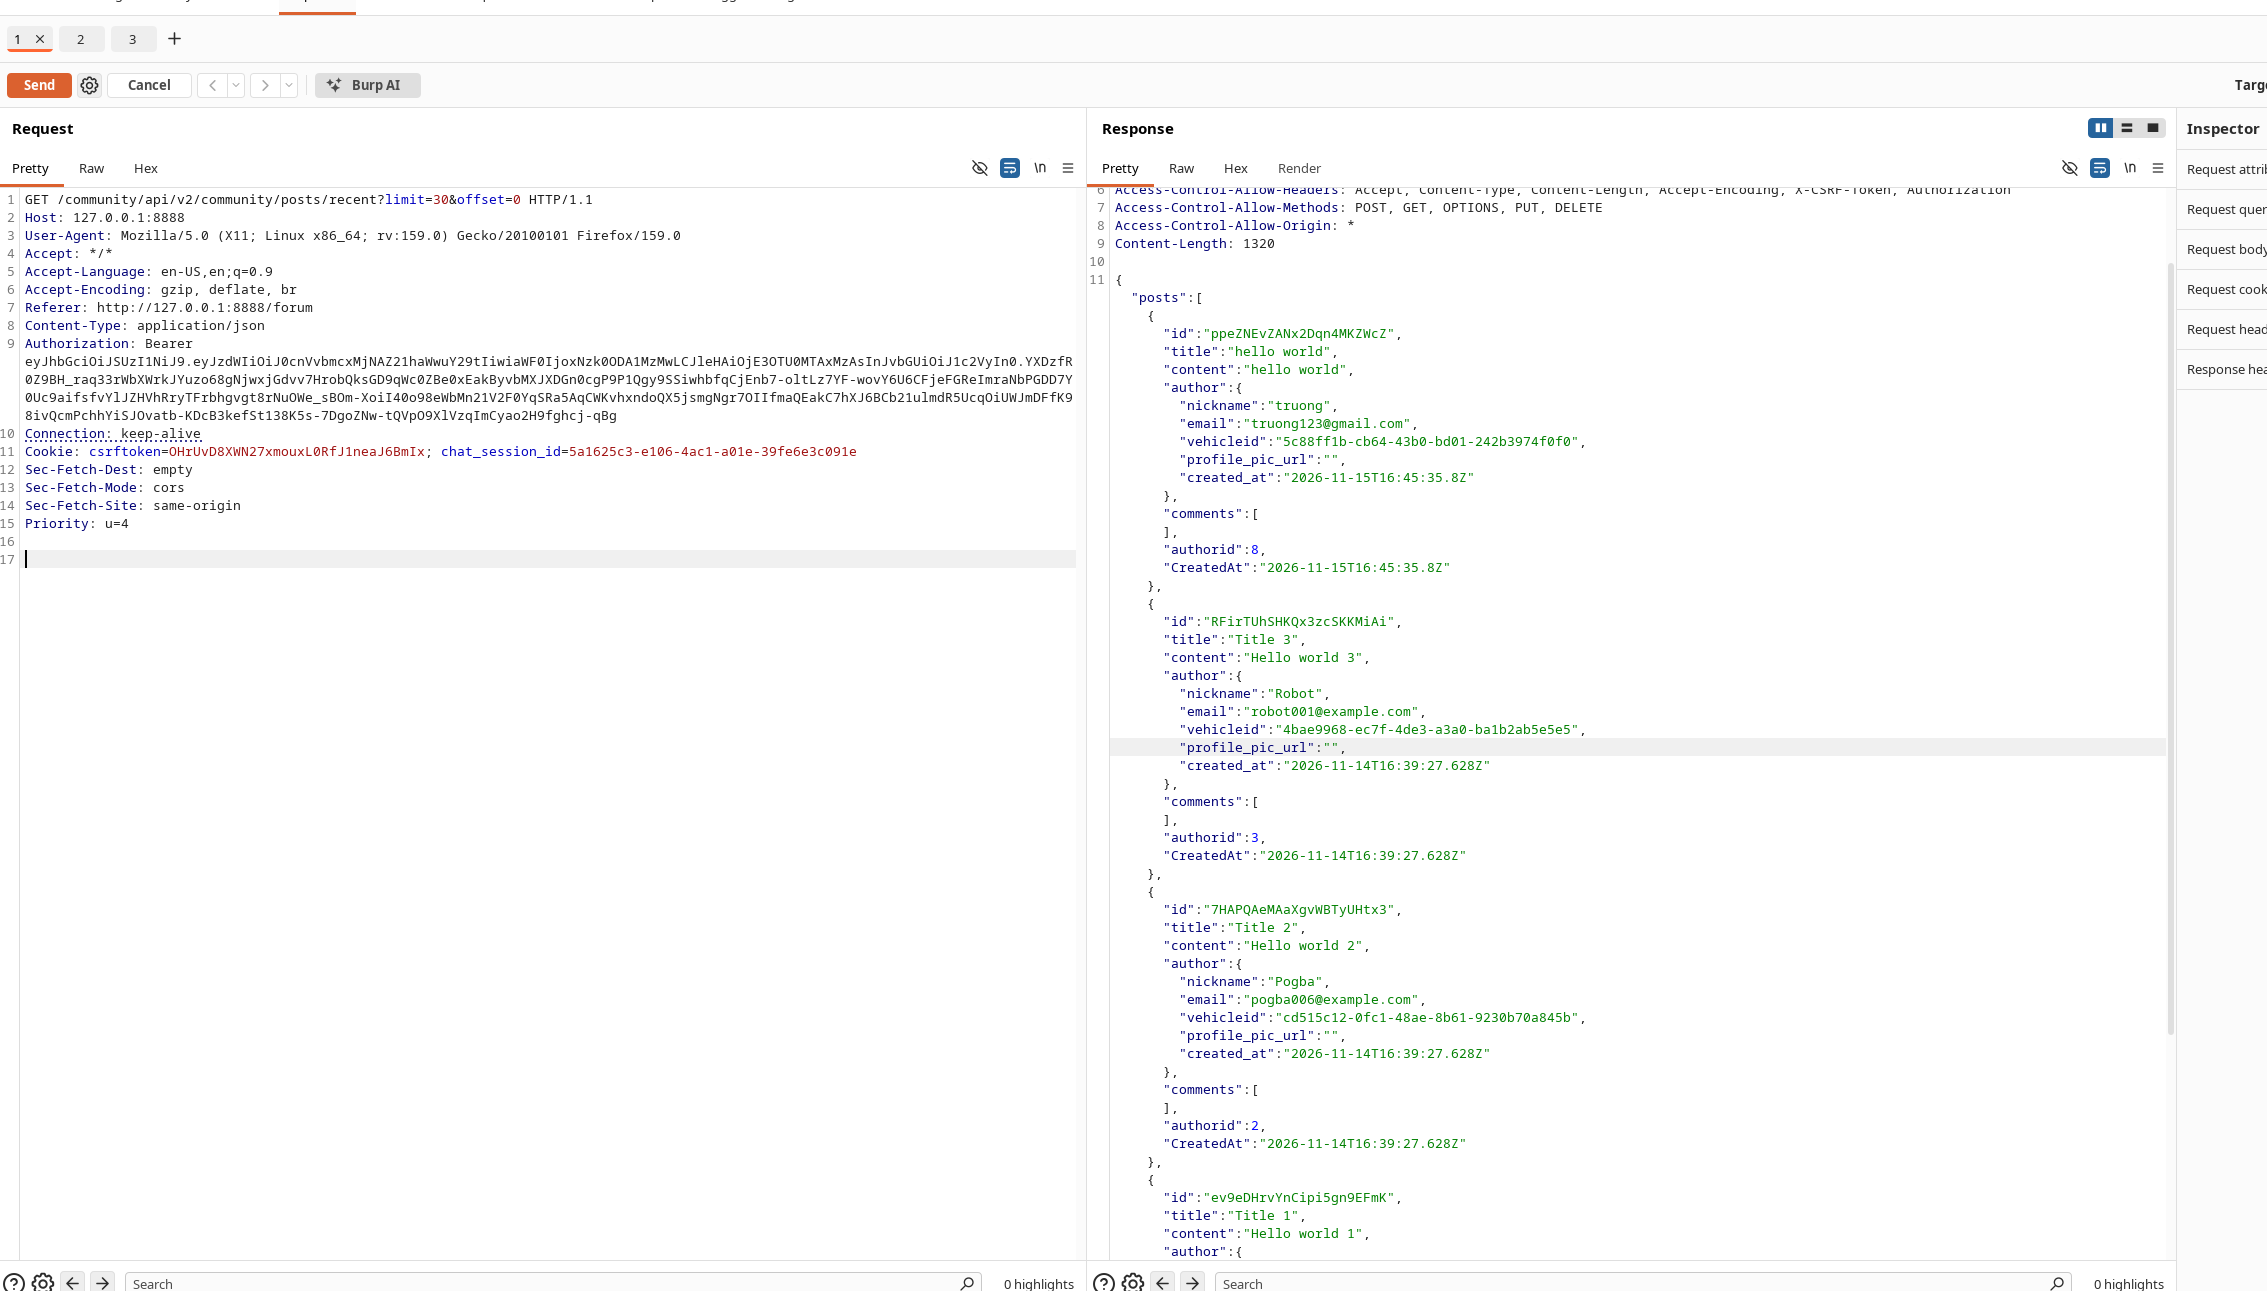
\includegraphics[width=\textwidth,height=0.52\textheight,keepaspectratio]{labs/03-data-exposure/evidence/endpoint-02-recent-posts/recent-posts.png}
    \caption{Danh sách bài viết chứa email và mã xe của tác giả.}
    \label{fig:exposure-recent}
\end{figure}


\begin{figure}[htbp]
    \centering
    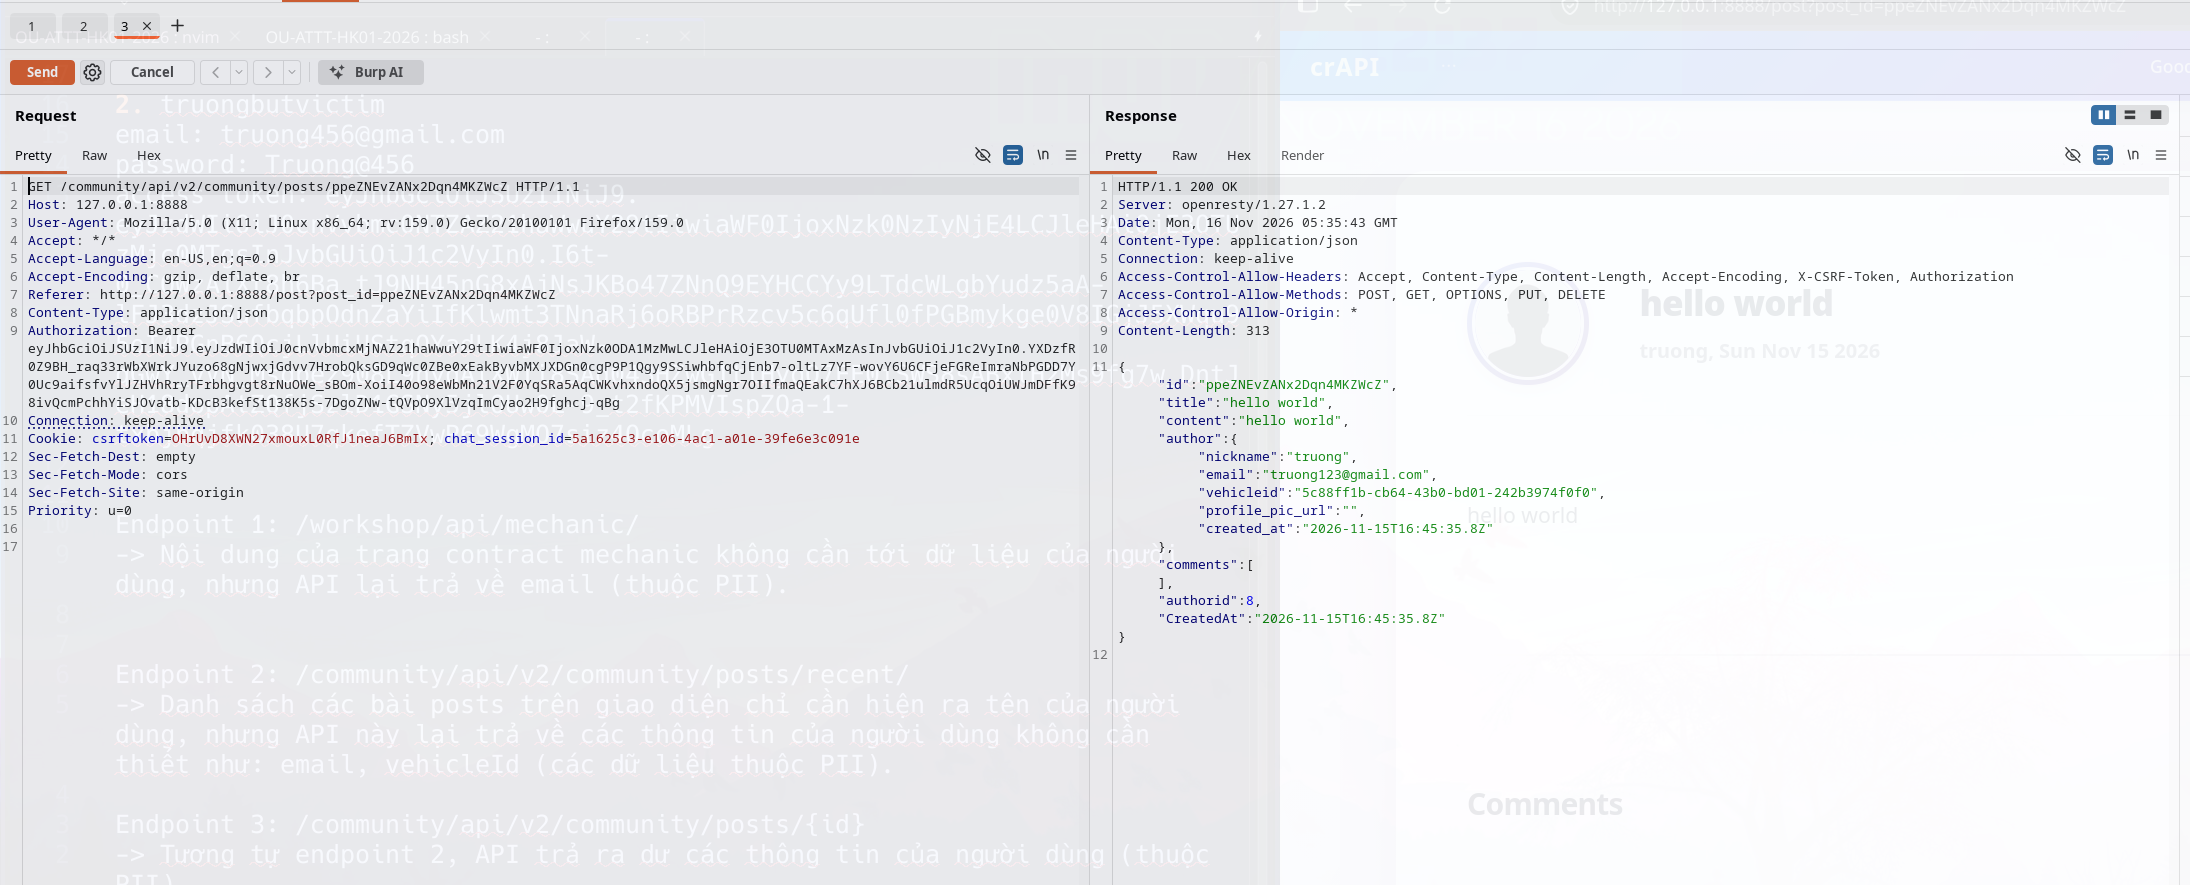
\includegraphics[width=\textwidth,height=0.52\textheight,keepaspectratio]{labs/03-data-exposure/evidence/endpoint-03-post-detail/post-detail.png}
    \caption{Chi tiết bài viết trả email và mã xe của tác giả.}
    \label{fig:exposure-detail}
\end{figure}


\clearpage
\subsection{Phản hồi sau khi gửi bình luận}
\begin{Verbatim}[breaklines=true,breakanywhere=true,fontsize=\small]
POST /community/api/v2/community/posts/{id}/comment
\end{Verbatim}

API trả lại bài viết cùng danh sách bình luận. Thông tin tác giả bài
viết và người bình luận đều có \texttt{email}, \texttt{vehicleid}.
Như vậy, những trường cần rà soát không chỉ xuất hiện khi đọc bảng tin
mà còn được gửi lại sau thao tác bình luận.


\begin{figure}[htbp]
    \centering
    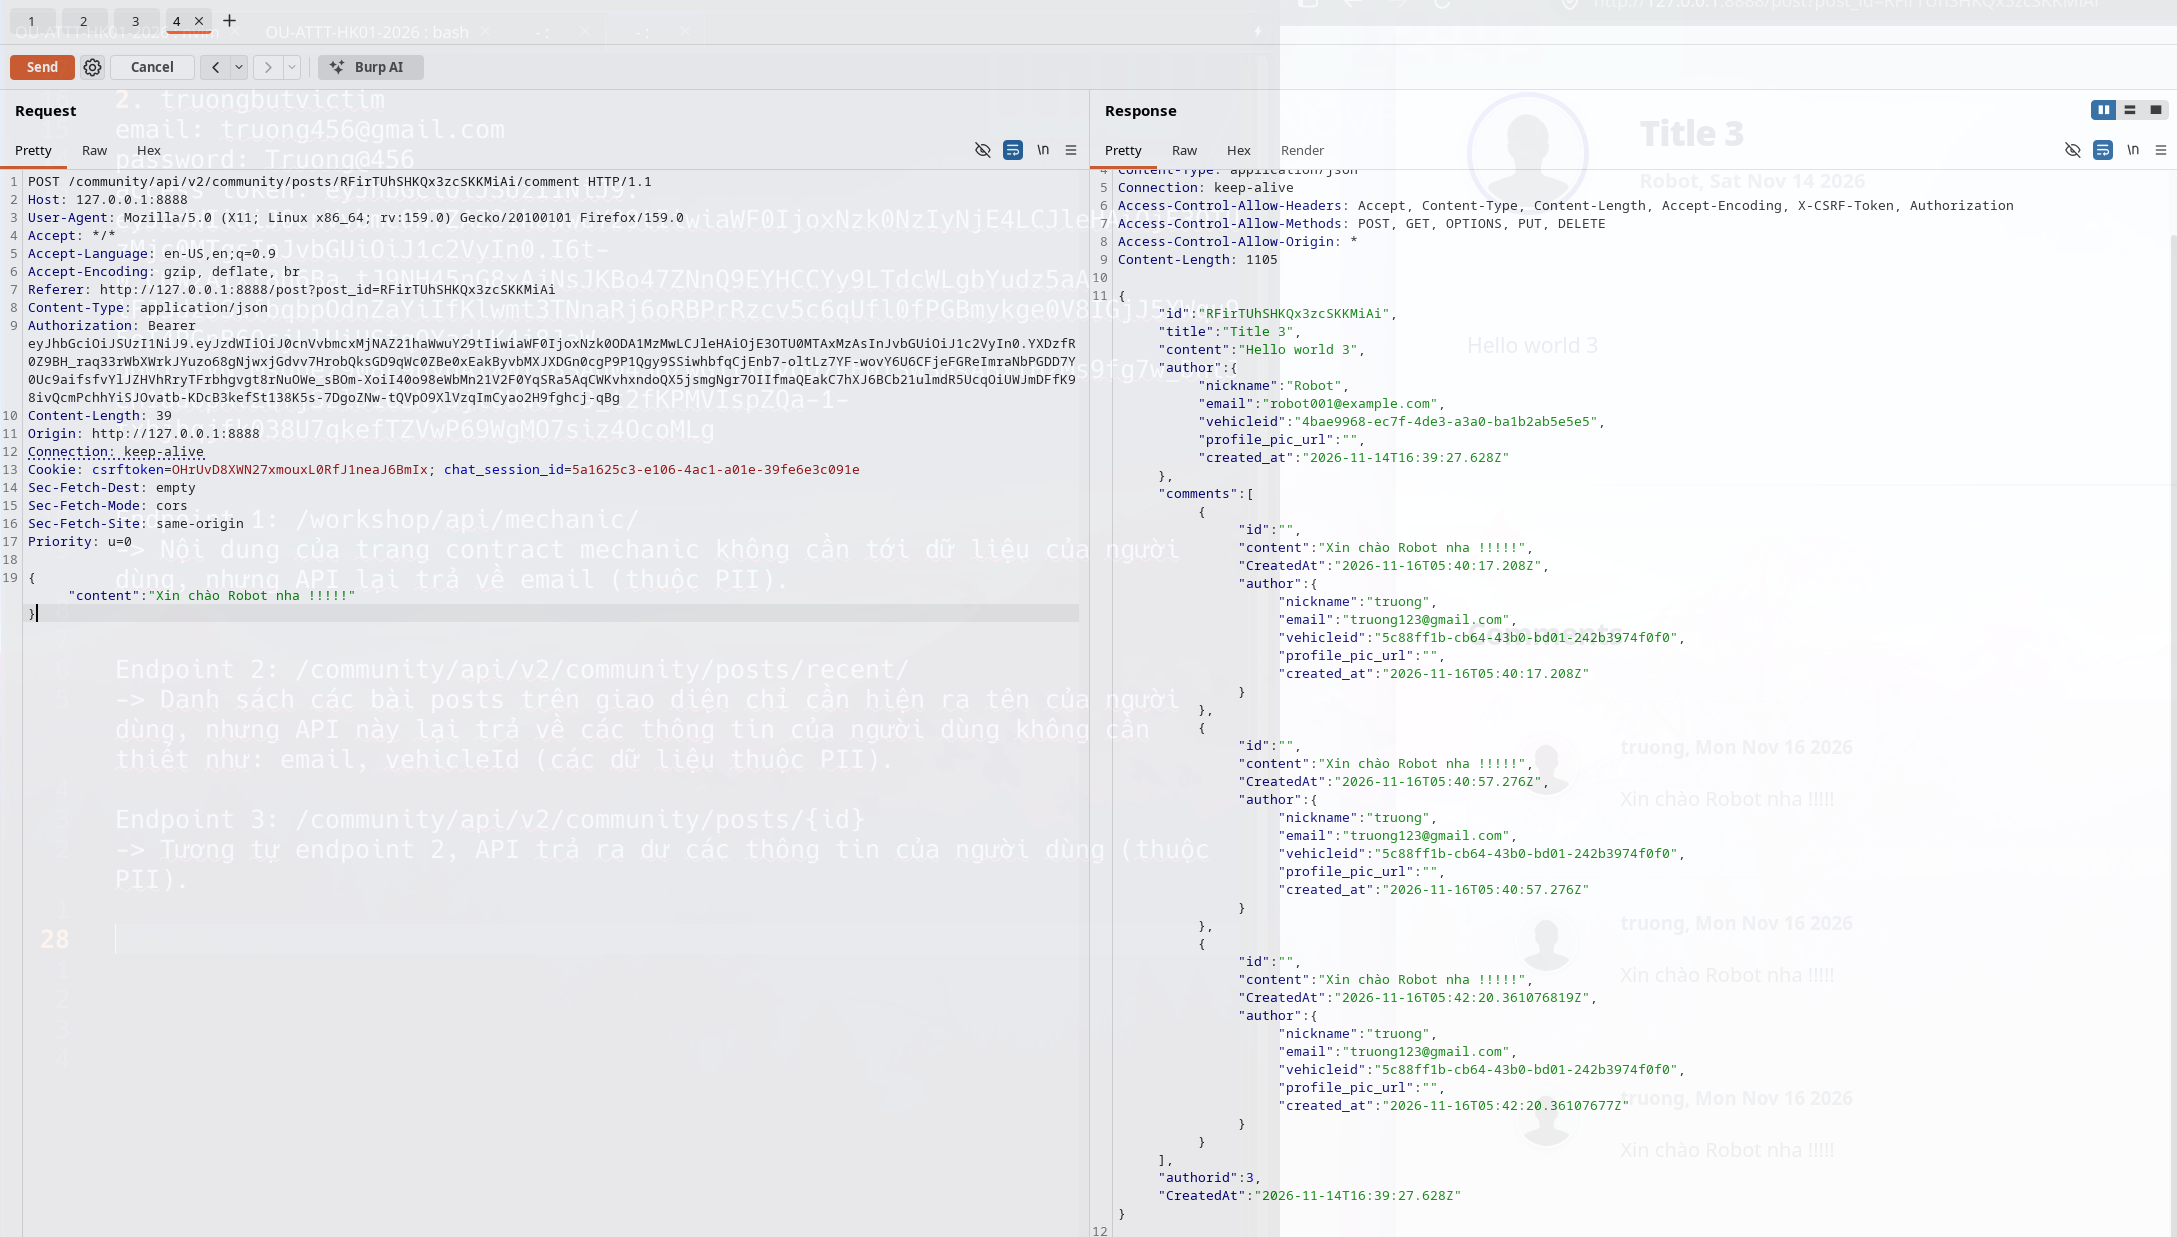
\includegraphics[width=\textwidth,height=0.52\textheight,keepaspectratio]{labs/03-data-exposure/evidence/endpoint-04-comments/comments.png}
    \caption{Phản hồi bình luận chứa thông tin tác giả bài viết và người bình luận.}
    \label{fig:exposure-comment}
\end{figure}


\subsection{Cập nhật ảnh đại diện}
\begin{Verbatim}[breaklines=true,breakanywhere=true,fontsize=\small]
POST /identity/api/v2/user/pictures
\end{Verbatim}

Sau khi tải ảnh lên, phản hồi có dữ liệu ảnh và trường
\texttt{available\_credit = 100.0}. Số dư không cần thiết để xác nhận
cập nhật ảnh thành công. Đây là số dư của tài khoản đang đăng nhập;
chưa chứng minh đọc được số dư người khác hoặc thay đổi được số dư.


\begin{figure}[htbp]
    \centering
    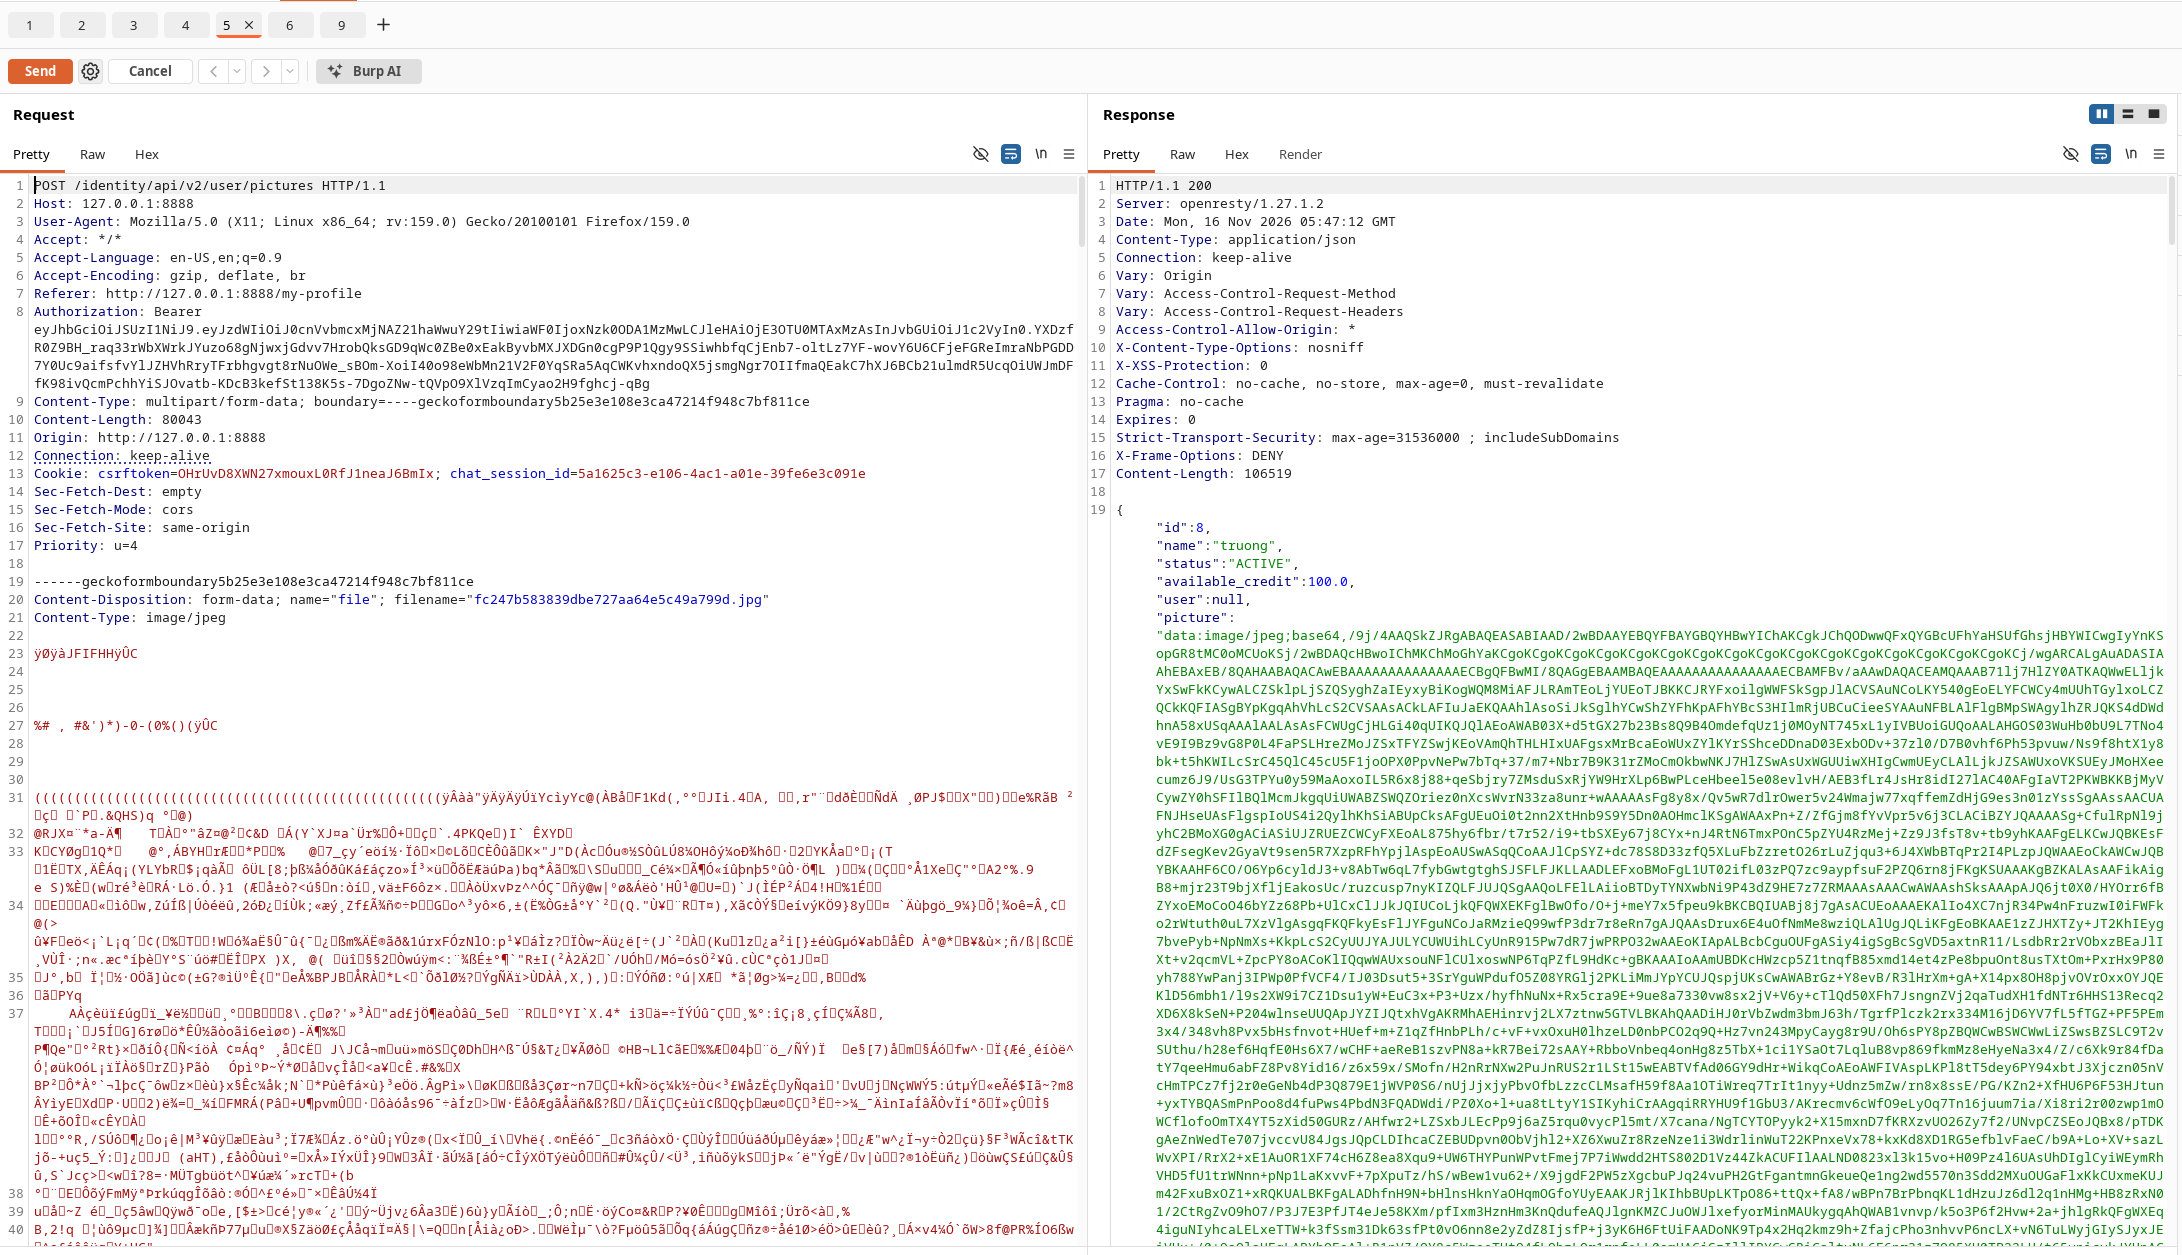
\includegraphics[width=\textwidth,height=0.52\textheight,keepaspectratio]{labs/03-data-exposure/evidence/endpoint-05-user-pictures/user-pictures.png}
    \caption{API đổi ảnh trả thêm available\_credit = 100.0.}
    \label{fig:exposure-picture}
\end{figure}


\clearpage
\subsection{Vị trí phương tiện}
\begin{Verbatim}[breaklines=true,breakanywhere=true,fontsize=\small]
GET /identity/api/v2/vehicle/{id}/location
\end{Verbatim}

Ngoài tọa độ, API trả thêm \texttt{fullName} và \texttt{email}. Cần
đánh giá hai trường này có cần thiết cho chức năng hiển thị bản đồ hay
không. Yêu cầu được ghi nhận là truy vấn xe của tài khoản thử nghiệm;
không dùng kết quả này để kết luận đã đọc trái phép xe người khác.


\begin{figure}[htbp]
    \centering
    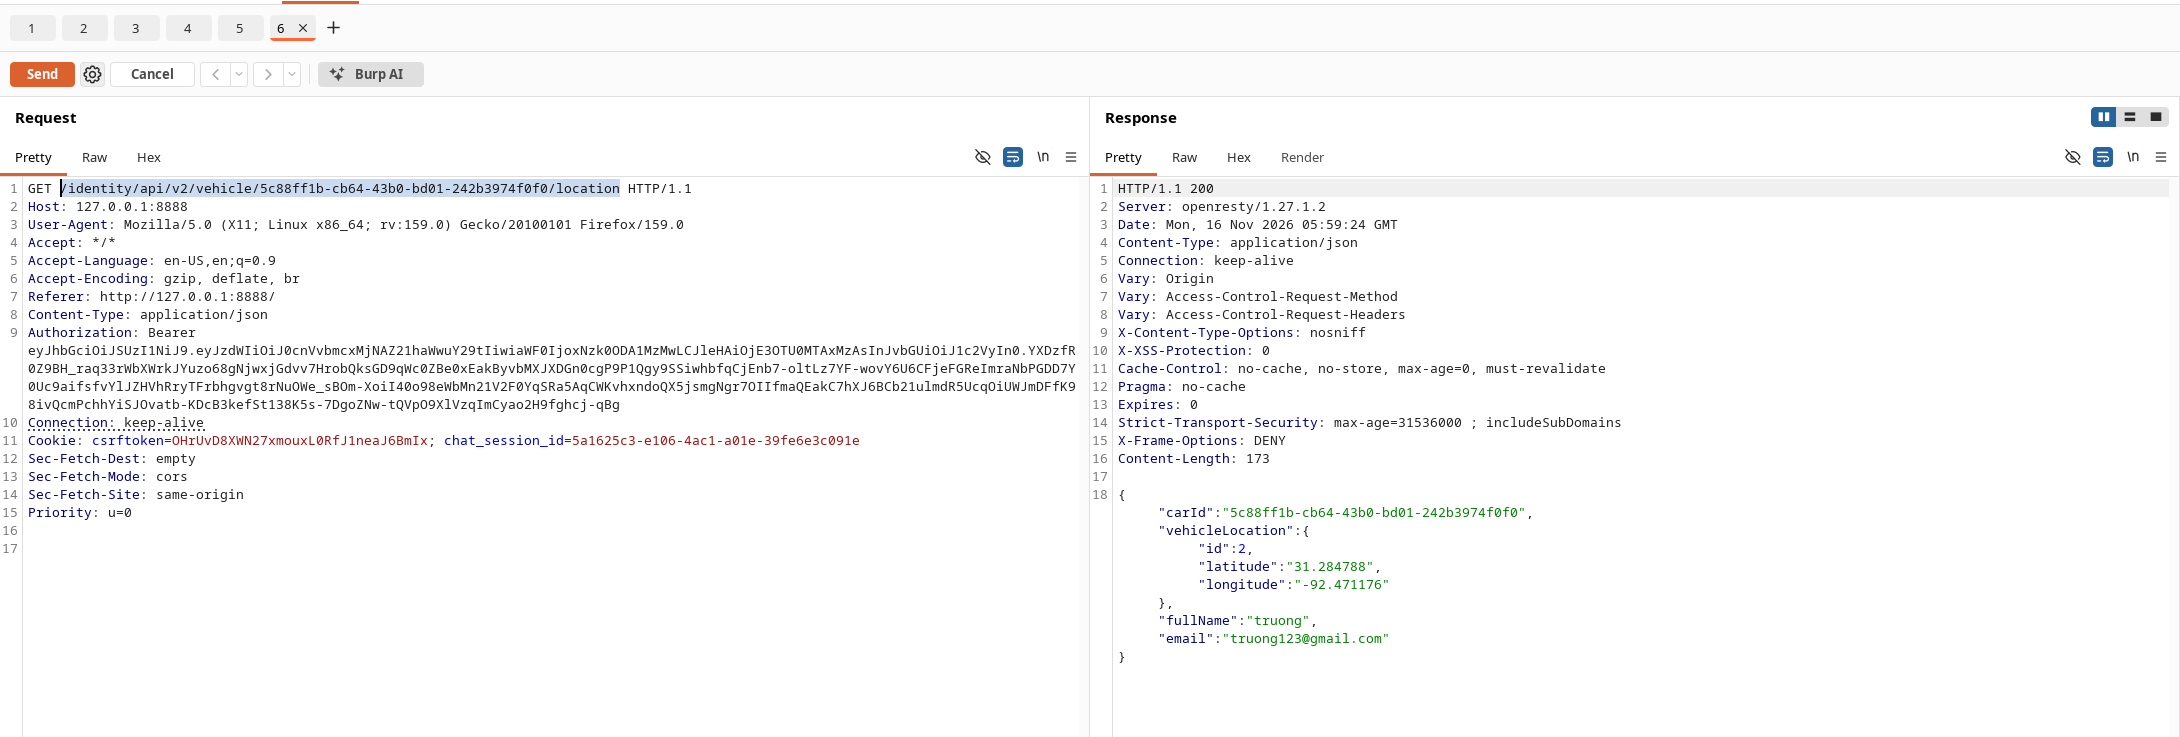
\includegraphics[width=\textwidth,height=0.52\textheight,keepaspectratio]{labs/03-data-exposure/evidence/endpoint-06-vehicle-location/vehicle-location.png}
    \caption{API vị trí xe trả fullName và email bên cạnh tọa độ.}
    \label{fig:exposure-location}
\end{figure}


\subsection{Danh sách phương tiện}
\begin{Verbatim}[breaklines=true,breakanywhere=true,fontsize=\small]
GET /identity/api/v2/vehicle/vehicles
\end{Verbatim}

Danh sách xe có trường \texttt{pincode}, giá trị \texttt{1080} trong
dữ liệu thử nghiệm. Mã này cần được kiểm soát chặt hơn các thuộc tính
mô tả xe như mẫu xe hoặc năm sản xuất. Bộ bằng chứng xác nhận mã xuất
hiện trong phản hồi, chưa xác nhận có thể dùng mã để chiếm xe hoặc tài
khoản khác.


\begin{figure}[htbp]
    \centering
    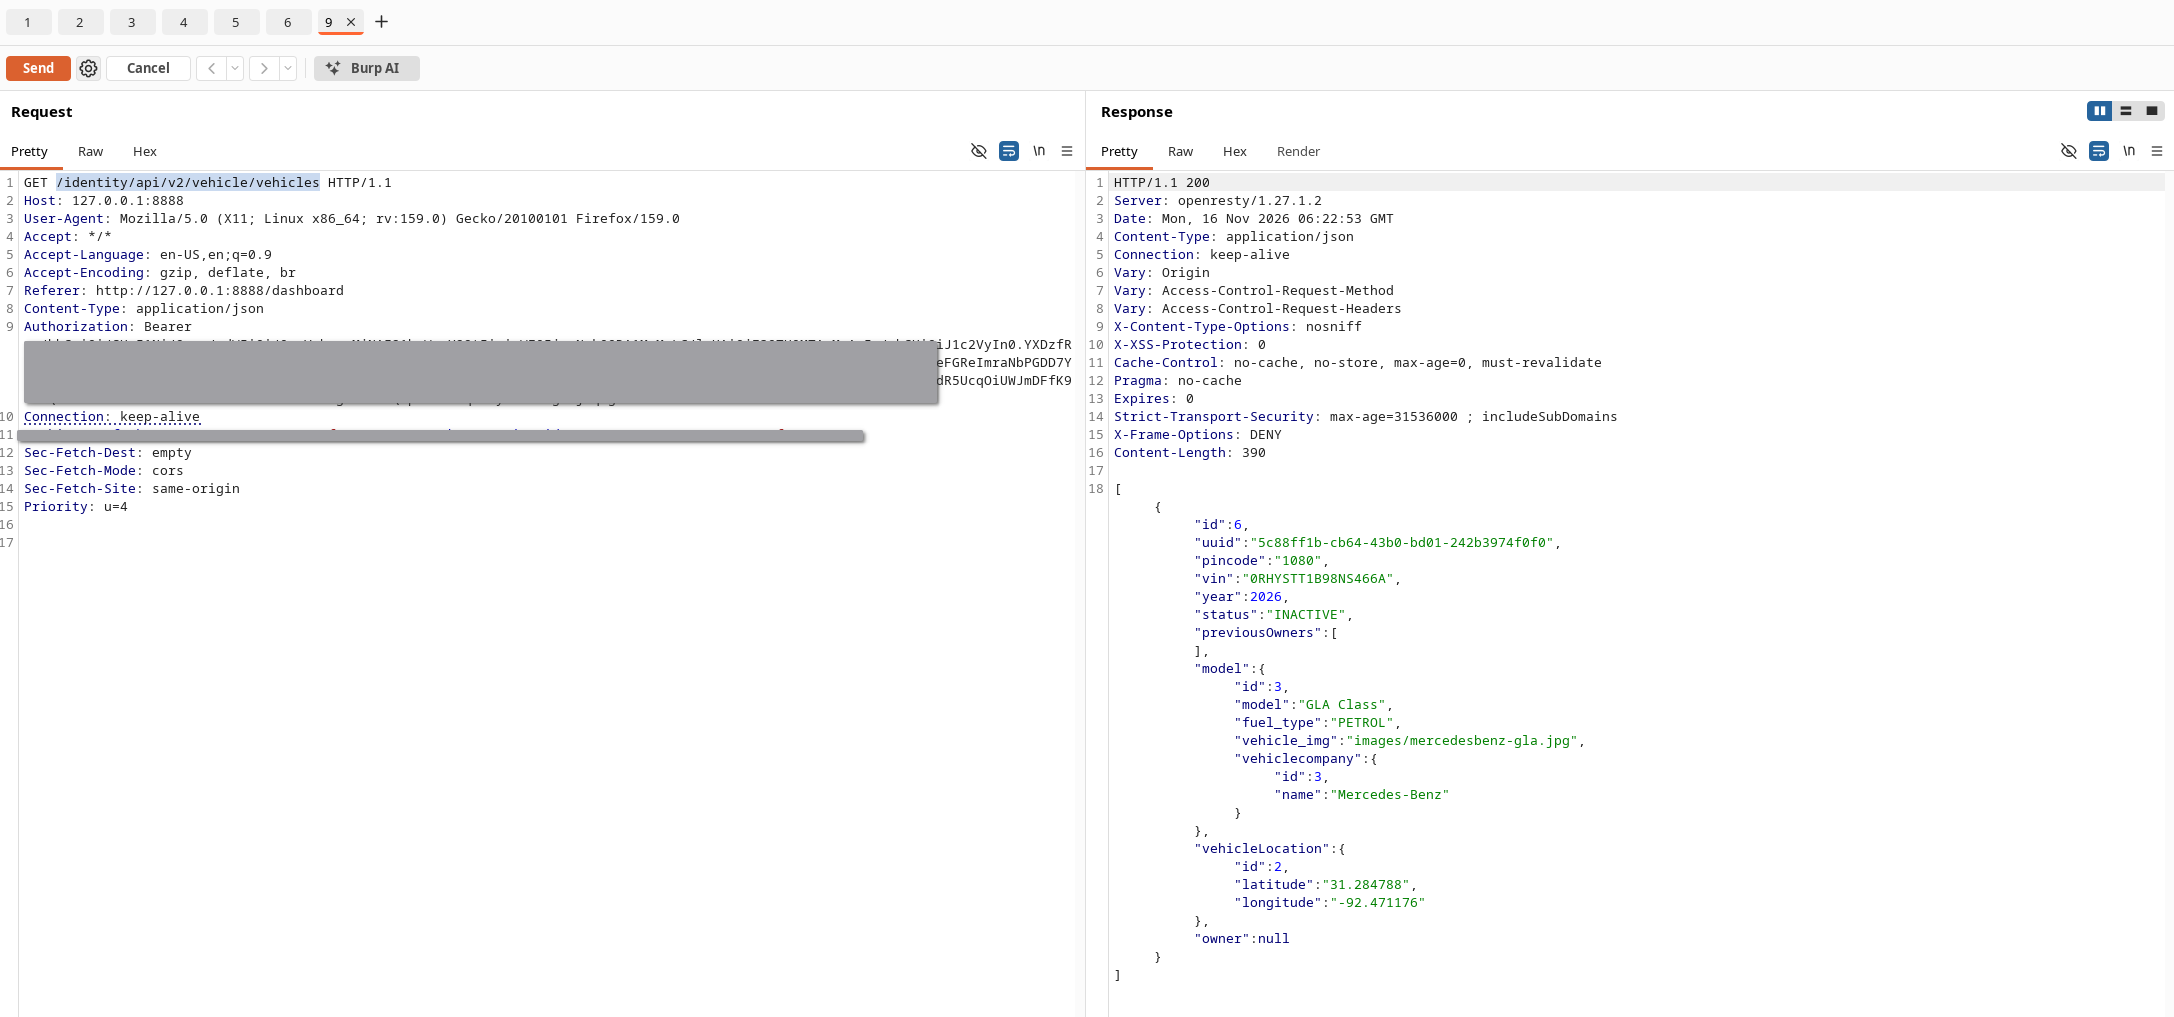
\includegraphics[width=\textwidth,height=0.52\textheight,keepaspectratio]{labs/03-data-exposure/evidence/endpoint-07-vehicles/vehicles.png}
    \caption{Danh sách xe có trường pincode.}
    \label{fig:exposure-vehicles}
\end{figure}


\clearpage
\section{Kiểm thử tự động}

File \path{tests/security/test_data_exposure.py} có bảy test tương ứng
bảy API. Mỗi test gọi API rồi duyệt các đối tượng và danh sách trong
JSON để tìm tên trường thuộc danh sách kiểm tra. Chạy bằng:
\begin{Verbatim}[breaklines=true,breakanywhere=true,fontsize=\small]
pytest -v tests/security/test_data_exposure.py
\end{Verbatim}

Tài khoản cần có xe để kiểm thử vị trí. Bộ test có thể tạo tài khoản,
bài viết, bình luận và tải ảnh đại diện, nên cần dùng dữ liệu thử
nghiệm riêng. Hồ sơ chưa có log pytest xác nhận kết quả chạy cả bảy bài.
Bảng~\ref{tab:exposure-tests} là phân loại dự kiến theo phản hồi đã lưu
và quy tắc hiện có trong mã test.

\begin{table}[htbp]
\centering
\caption{Các trường được kiểm tra và phân loại dự kiến của bộ test}
\label{tab:exposure-tests}
\begin{tabularx}{\textwidth}{@{} p{0.26\textwidth} X l @{}}
\toprule
\textbf{Chức năng} & \textbf{Trường cần kiểm tra} & \textbf{Phân loại} \\
\midrule
Thợ sửa xe & \texttt{email}, \texttt{number} & WARNING \\
Danh sách bài viết & \texttt{email}, \texttt{vehicleid} & WARNING \\
Chi tiết bài viết & \texttt{email}, \texttt{vehicleid} & WARNING \\
Gửi bình luận & \texttt{email}, \texttt{vehicleid} & WARNING \\
Đổi ảnh đại diện & \texttt{available\_credit} & FAILED \\
Vị trí xe & \texttt{fullName}, \texttt{email} & WARNING \\
Danh sách xe & \texttt{pincode} & FAILED \\
\bottomrule
\end{tabularx}
\end{table}

WARNING là cảnh báo do test phát ra, không phải trạng thái riêng của
pytest; test vẫn có thể PASSED nếu chỉ có cảnh báo. FAILED do trường
bị cấm cần được phân biệt với lỗi đăng nhập, gọi API hoặc thiếu dữ liệu.

Test tìm theo tên trường, kể cả khi giá trị rỗng. Do đó, các nhãn trên
phản ánh quy tắc của bộ test, không phải kết luận mức độ nghiêm trọng
chung cho mọi tình huống. Chẳng hạn, nhận số dư của chính mình khi đổi
ảnh không chứng minh số dư của người khác bị lộ.

\section{Nguyên nhân, tác động và cách khắc phục}

Điểm chung được quan sát là phản hồi chứa thông tin ngoài nhu cầu chức
năng. Một nguyên nhân có thể là dùng chung cấu trúc phản hồi hoặc trả
toàn bộ đối tượng người dùng. Đây là hướng cần kiểm tra ở lớp tạo JSON;
hồ sơ chưa xác định dòng mã backend gây ra từng trường hợp.

Trong dữ liệu Community, người dùng nhận thêm email và mã xe của các
tác giả khác. Những thông tin này có thể hỗ trợ thu thập dữ liệu cá
nhân hoặc tìm đối tượng để kiểm thử truy cập trái phép. Chưa có bằng
chứng về chiếm quyền tài khoản hoặc gian lận tiền từ các dữ liệu đã thấy.

Các biện pháp đề xuất gồm:
\begin{enumerate}
    \item Quy định trường được trả về cho từng API theo chức năng và
    quyền người nhận. Dùng cấu trúc phản hồi riêng thay vì trả toàn bộ
    đối tượng dữ liệu.
    \item Loại bỏ email và mã xe khỏi bài viết, bình luận nếu không cần
    dùng; không trả số dư trong chức năng đổi ảnh. Kiểm soát riêng quyền
    nhận mã PIN của xe.
    \item Lọc dữ liệu tại máy chủ. Việc không hiển thị trên giao diện
    không ngăn người dùng đọc dữ liệu từ phản hồi API.
    \item Sau khi sửa, gửi lại các yêu cầu đã lưu, xác nhận dữ liệu thừa
    được loại bỏ và chức năng hợp lệ vẫn hoạt động. Cập nhật test theo
    danh sách trường được phép của từng API.
\end{enumerate}

Lab ghi nhận các trường cần rà soát ở bảy phản hồi API, trong đó
Community có thông tin của tác giả khác tài khoản đang đăng nhập.
Chưa có bản vá hoặc kết quả kiểm thử sau vá trong bộ bằng chứng.

\clearpage
\chapter{Lab 04: Sửa trạng thái đơn hàng để được hoàn tiền (Mass Assignment)}
\label{chap:lab04}

\section{Bài toán và mục tiêu kiểm thử}

Khi mua hàng trong Shop của crAPI, người dùng thanh toán bằng số dư tài
khoản. Nếu muốn trả hàng, người dùng chỉ nên được tạo yêu cầu trả hàng;
việc xác nhận đã trả hàng và hoàn tiền phải do máy chủ kiểm soát.
Lab này kiểm tra xem người dùng có thể tự đổi trạng thái đơn hàng thành
đã trả hàng để được cộng lại tiền hay không.

Lỗi được khảo sát là \textbf{Mass Assignment}: API cho phép phía người
dùng sửa thuộc tính mà họ không có quyền quyết định. Trong trường hợp
này, thuộc tính đó là \texttt{status} (trạng thái đơn hàng). Lỗi thuộc
nhóm thiếu kiểm soát quyền trên thuộc tính đối tượng
(\textit{Broken Object Property Level Authorization})~\cite{owasp-property}.

Khác với Lab 01, người kiểm thử thao tác trên đơn hàng của chính mình.
Vấn đề cần kiểm tra là quyền thay đổi trạng thái hoàn tiền, không phải
quyền truy cập đơn hàng của người khác.

\section{Chuẩn bị và hành vi mong đợi}

Thực nghiệm sử dụng tài khoản thử nghiệm trên crAPI cục bộ tại
\url{http://127.0.0.1:8888}. Burp Suite được dùng để quan sát yêu cầu
mua hàng và gửi yêu cầu đã chỉnh sửa qua Repeater.

Sản phẩm được chọn là Wheel, giá \texttt{10.00}, số lượng \texttt{1}.
Tài khoản có số dư ban đầu là \texttt{100.0}. Sau khi mua, số dư còn
\texttt{90.0}; đơn hàng được tạo có mã \texttt{15}.

Đối chiếu mã nguồn cho thấy chức năng yêu cầu trả hàng đưa đơn về trạng
thái \texttt{return pending} (chờ xử lý trả hàng). Một hệ thống an toàn
chỉ được chuyển sang \texttt{returned} (đã trả hàng) và hoàn tiền sau
khi xác minh đủ điều kiện. Người dùng không được tự gán trạng thái này
qua API cập nhật đơn hàng~\cite{crapi-shop}.

\section{Các bước kiểm thử và kết quả}

\subsection{Mua hàng và ghi nhận dữ liệu trước kiểm thử}

Trên giao diện Shop, số dư giảm từ 100 xuống 90 sau khi mua một Wheel
(Hình~\ref{fig:mass-shop-before} và Hình~\ref{fig:mass-shop-after}).

\begin{figure}[htbp]
    \centering
    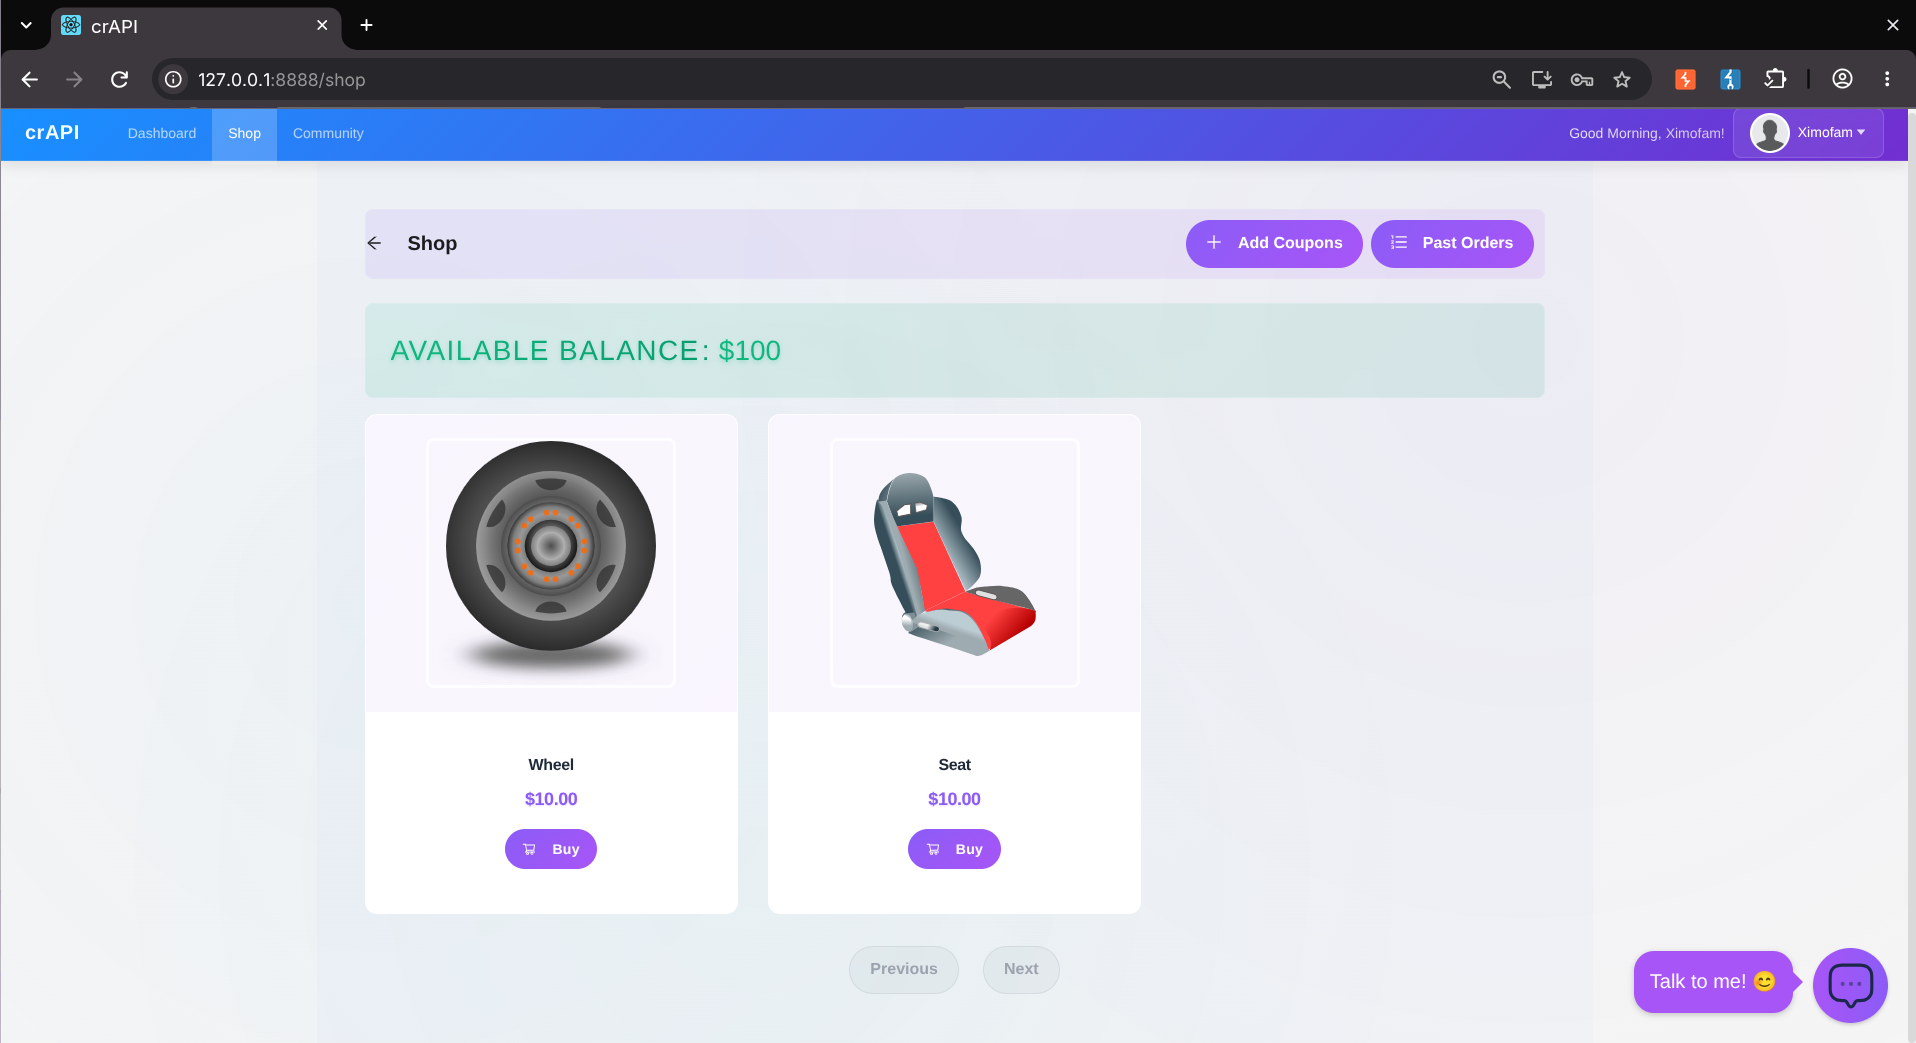
\includegraphics[width=\textwidth,height=0.52\textheight,keepaspectratio]{labs/04-mass-assignment/evidence/01-shop-before.png}
    \caption{Shop trước khi mua: số dư 100, sản phẩm Wheel giá 10.}
    \label{fig:mass-shop-before}
\end{figure}

\begin{figure}[htbp]
    \centering
    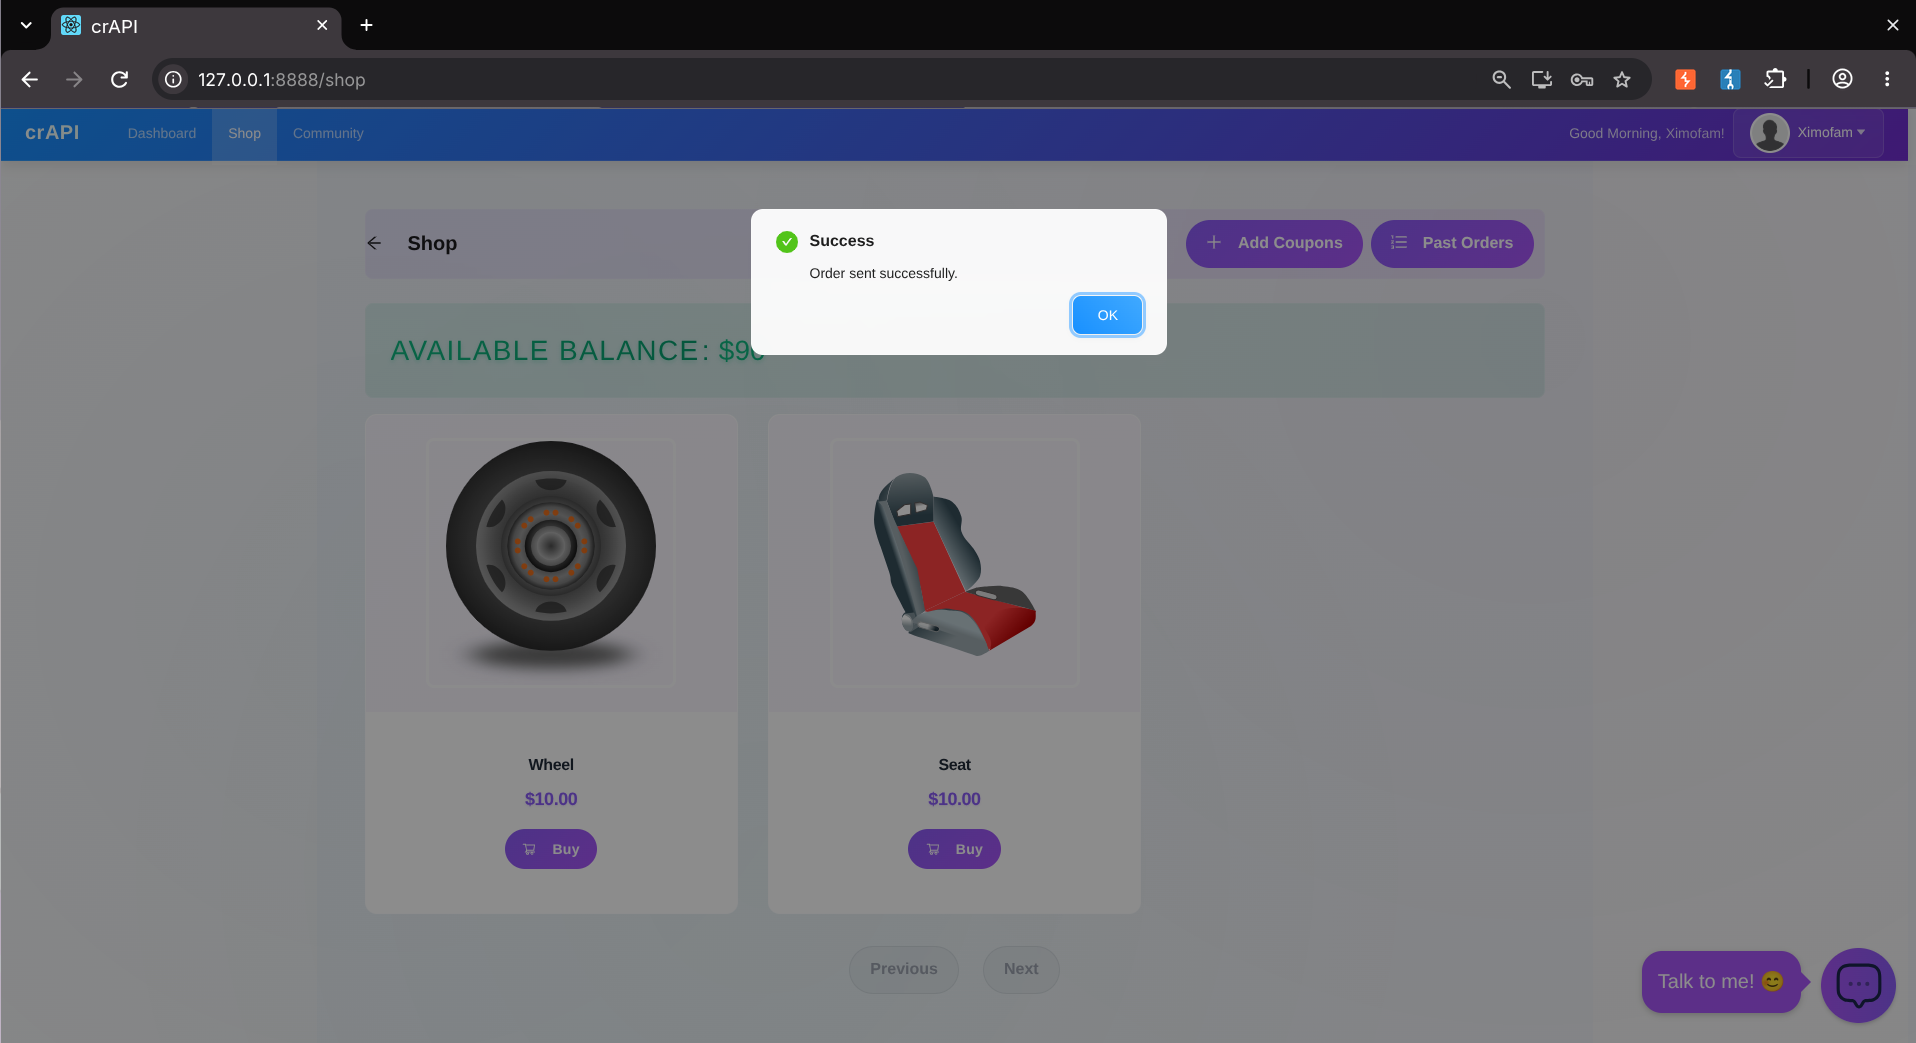
\includegraphics[width=\textwidth,height=0.52\textheight,keepaspectratio]{labs/04-mass-assignment/evidence/02-shop-after.png}
    \caption{Shop sau khi mua Wheel: số dư còn 90.}
    \label{fig:mass-shop-after}
\end{figure}

Tại Shop, mua một Wheel. Yêu cầu tạo đơn hàng được ghi nhận như sau;
thông tin xác thực đã được ẩn:

\begin{Verbatim}[breaklines=true,breakanywhere=true,fontsize=\small]
POST /workshop/api/shop/orders HTTP/1.1
Host: 127.0.0.1:8888
Authorization: Bearer <REDACTED>
Content-Type: application/json

{"product_id": 2, "quantity": 1}
\end{Verbatim}

Máy chủ trả \texttt{HTTP 200}, xác nhận mã đơn \texttt{15} và số dư
\texttt{90.0}. Sau đó, đọc lại dữ liệu bằng hai yêu cầu GET:

\begin{Verbatim}[breaklines=true,breakanywhere=true,fontsize=\small]
GET /workshop/api/shop/products?limit=30&offset=0
GET /workshop/api/shop/orders/all?limit=30&offset=0
\end{Verbatim}

Phản hồi thứ nhất xác nhận số dư \texttt{90.0}. Phản hồi thứ hai xác
nhận đơn \texttt{15} có số lượng \texttt{1}, trạng thái
\texttt{delivered} (đã giao). Đây là dữ liệu đối chiếu trước khi sửa
trạng thái, được đọc từ API thay vì chỉ dựa vào giao diện.



\begin{figure}[htbp]
    \centering
    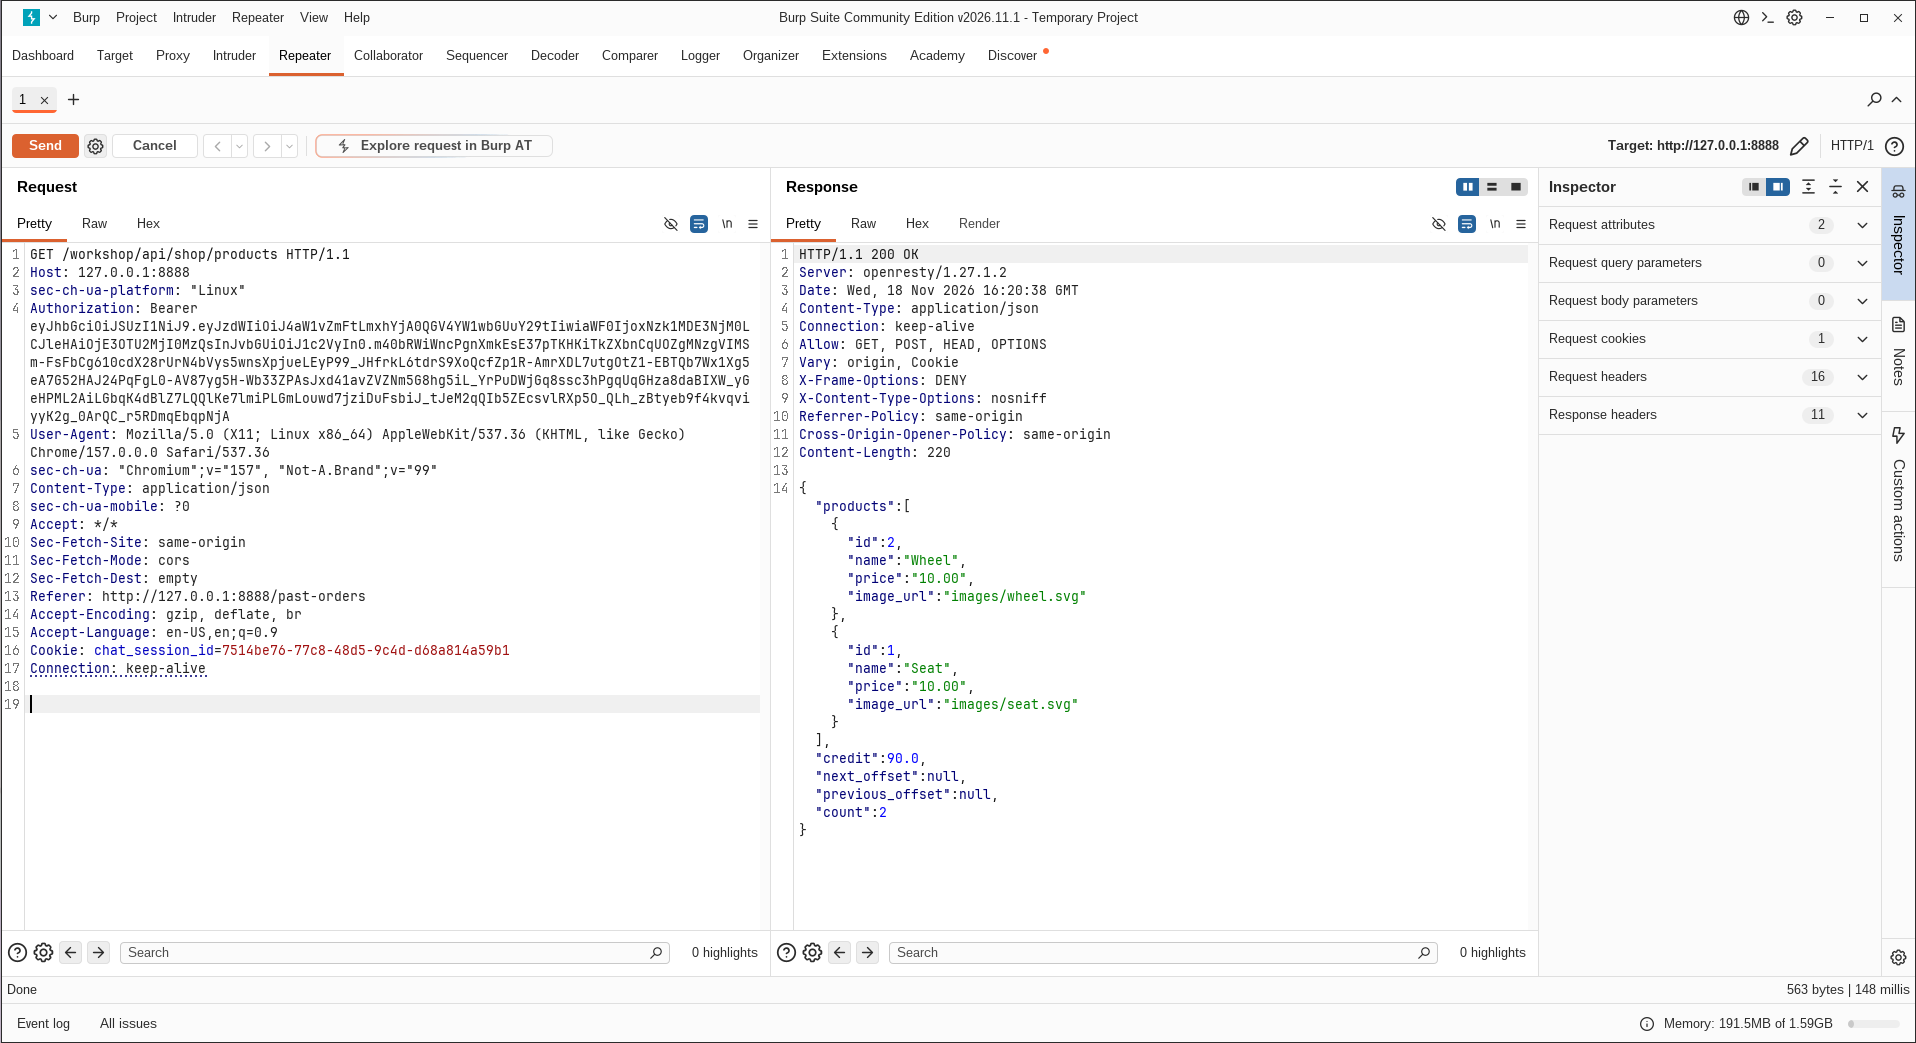
\includegraphics[width=\textwidth,height=0.52\textheight,keepaspectratio]{labs/04-mass-assignment/evidence/06-credit-before-put.png}
    \caption{GET products trước PUT: API trả số dư 90.0.}
    \label{fig:mass-credit-before}
\end{figure}

\begin{figure}[htbp]
    \centering
    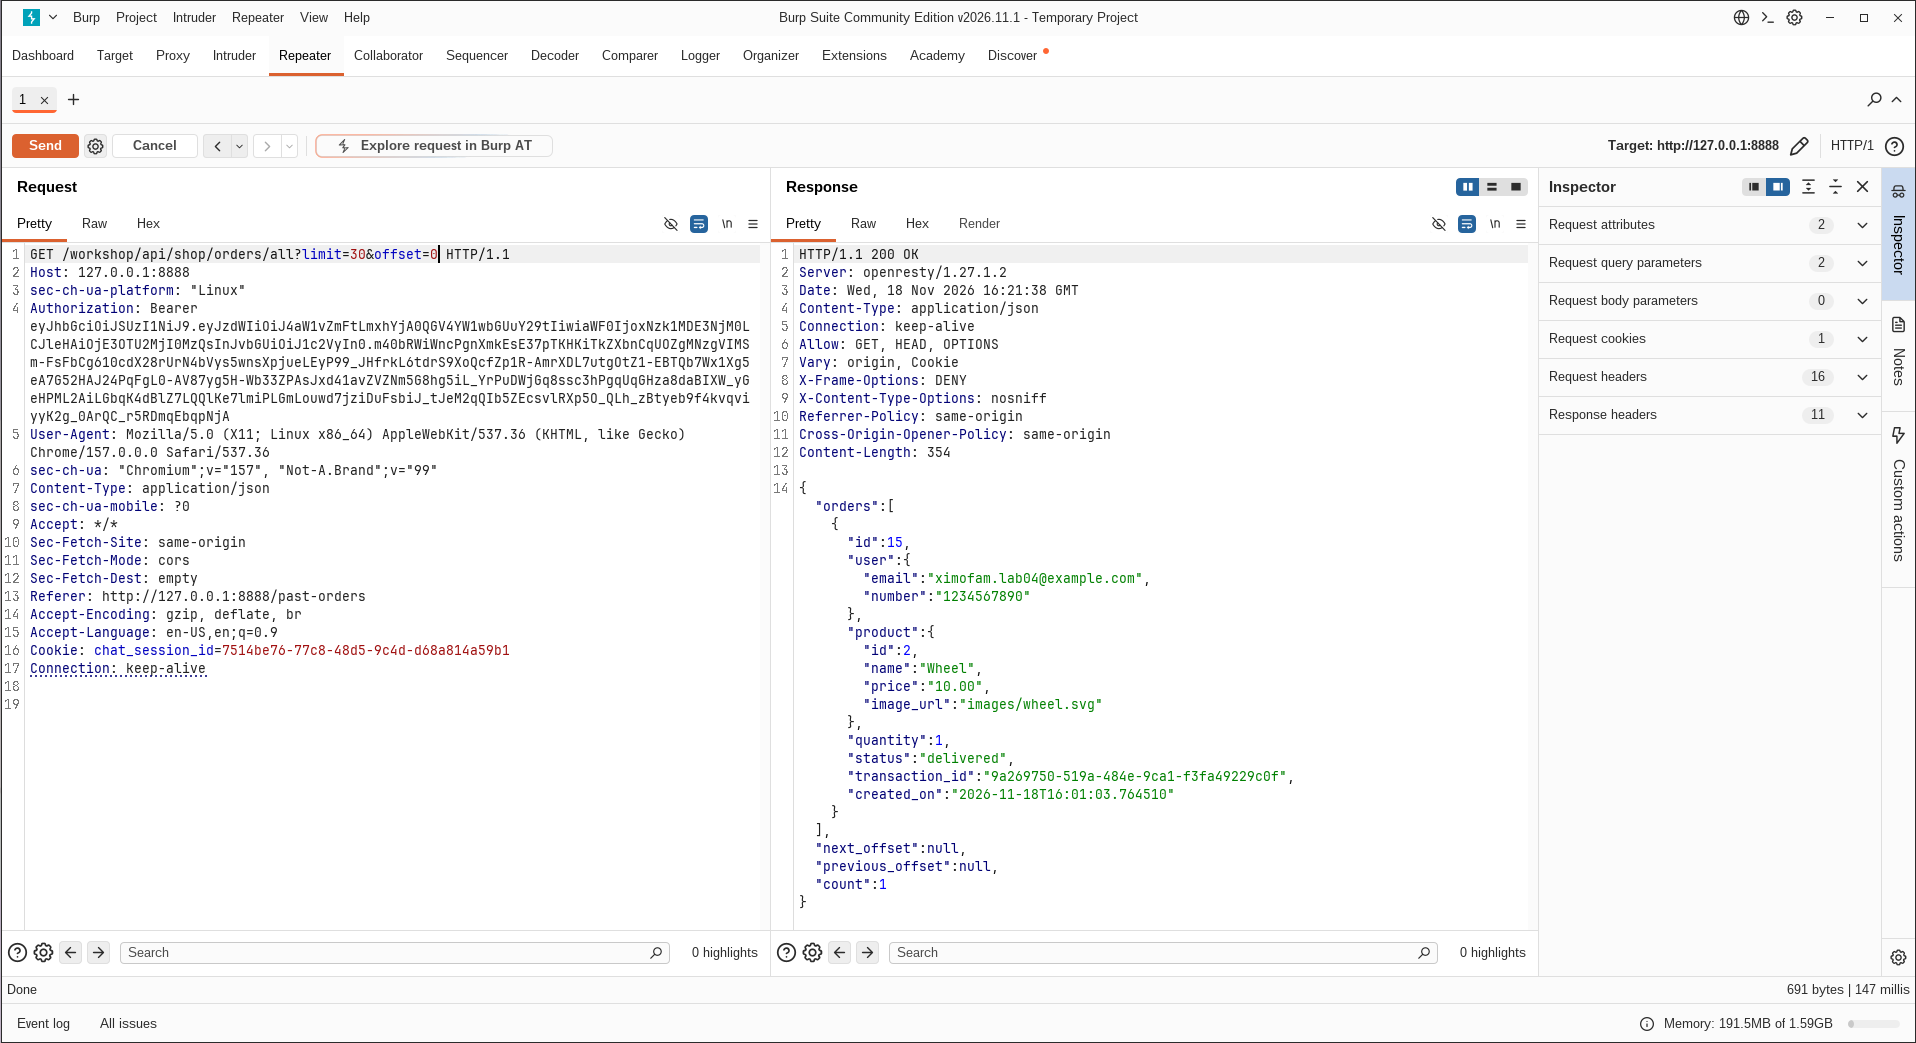
\includegraphics[width=\textwidth,height=0.52\textheight,keepaspectratio]{labs/04-mass-assignment/evidence/07-order-before-put.png}
    \caption{GET orders trước PUT: đơn 15 có trạng thái delivered.}
    \label{fig:mass-order-before}
\end{figure}

\clearpage
\subsection{Gửi yêu cầu đổi trạng thái đơn hàng}

Trong Burp Repeater, sử dụng phiên đăng nhập của chủ đơn hàng và gửi:

\begin{Verbatim}[breaklines=true,breakanywhere=true,fontsize=\small]
PUT /workshop/api/shop/orders/15 HTTP/1.1
Host: 127.0.0.1:8888
Authorization: Bearer <REDACTED>
Content-Type: application/json

{"status": "returned"}
\end{Verbatim}

Yêu cầu này trực tiếp gán trạng thái đã trả hàng. Nội dung gửi lên không
có thông tin xác minh việc trả hàng. Máy chủ trả \texttt{HTTP 200} và
phản hồi đơn \texttt{15} với \texttt{status = returned}.


\begin{figure}[htbp]
    \centering
    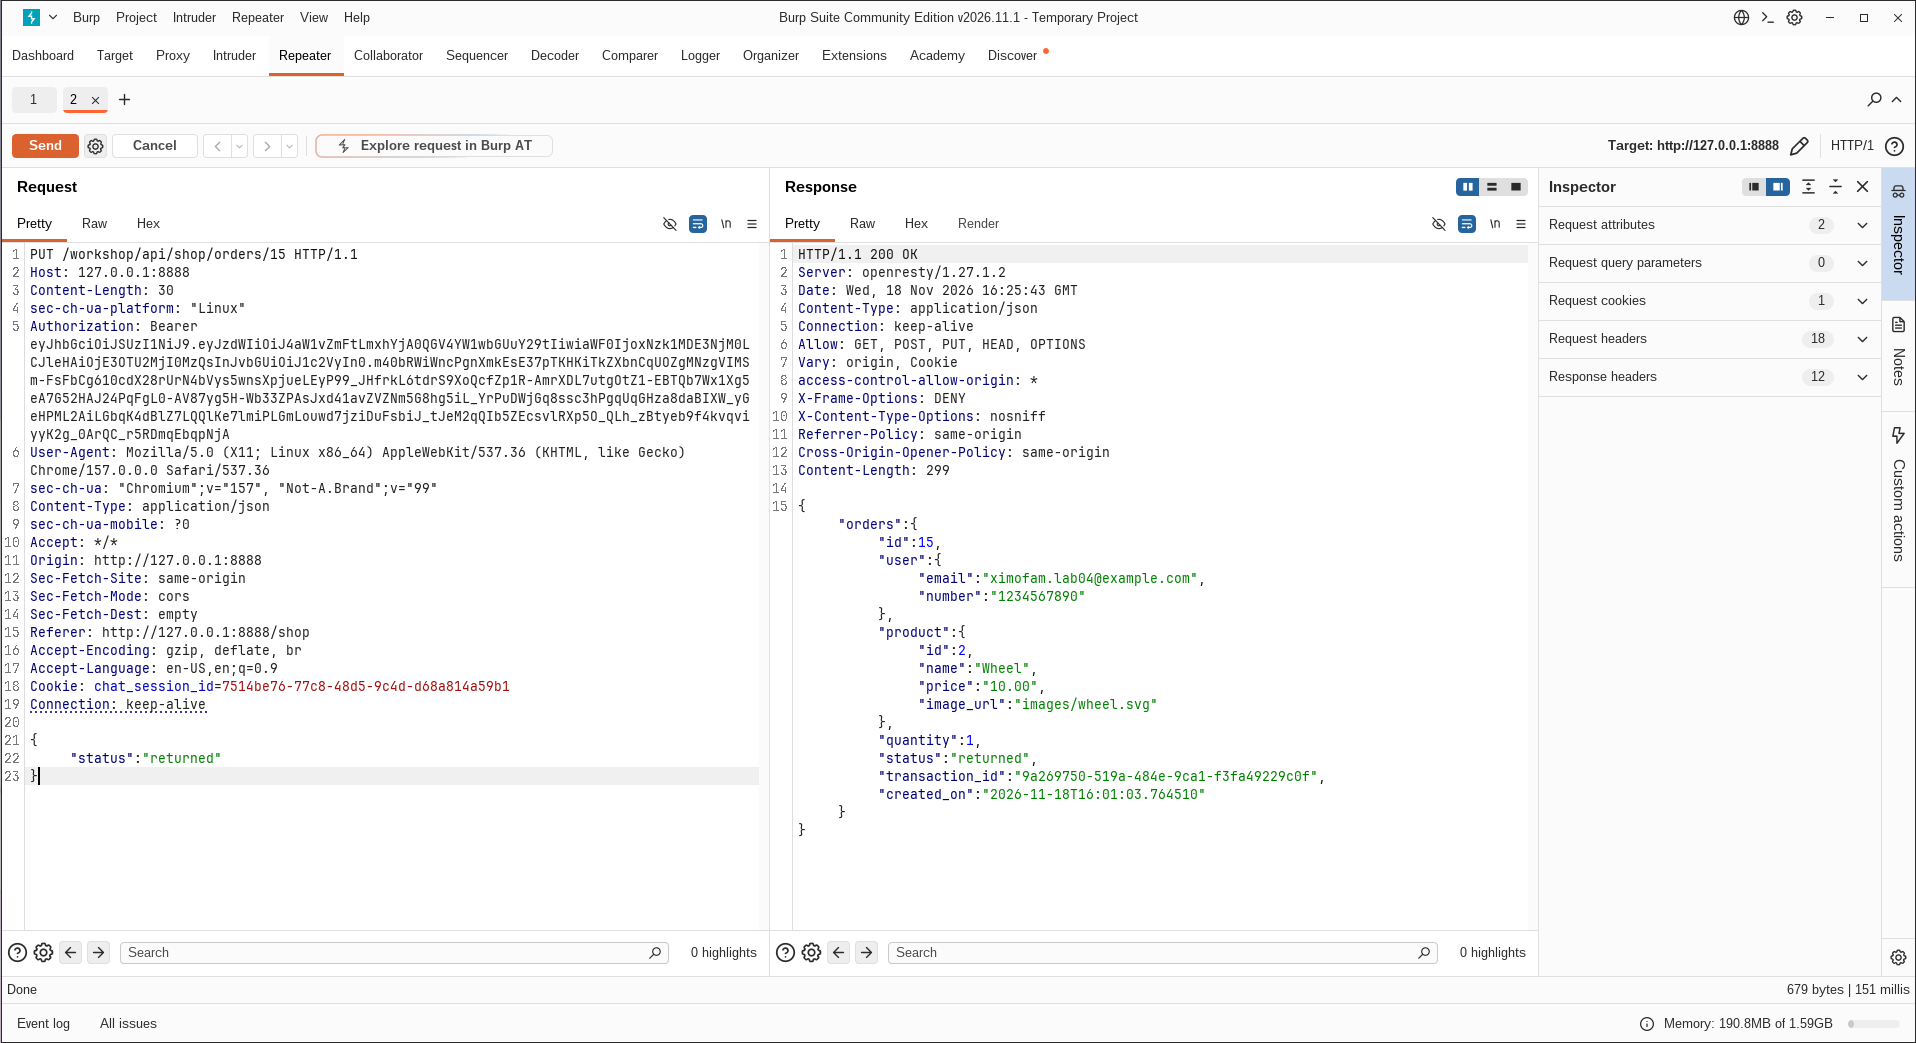
\includegraphics[width=\textwidth,height=0.52\textheight,keepaspectratio]{labs/04-mass-assignment/evidence/08-put-status-returned.png}
    \caption{Burp Repeater: gửi status = returned, API trả HTTP 200 và trạng thái returned.}
    \label{fig:mass-put}
\end{figure}

\clearpage
\subsection{Đọc lại trạng thái và số dư}

Để xác định thay đổi có được lưu thực sự hay không, gửi lại hai yêu cầu
GET lấy danh sách sản phẩm và đơn hàng. Các trường liên quan trong phản
hồi được trích như sau; đây là hai phản hồi riêng:

\begin{Verbatim}[breaklines=true,breakanywhere=true,fontsize=\small]
// GET products: so du sau PUT
{"credit": 100.0}

// GET orders/all: don hang sau PUT
{
  "id": 15,
  "product": {"id": 2, "name": "Wheel", "price": "10.00"},
  "quantity": 1,
  "status": "returned"
}
\end{Verbatim}


\begin{figure}[htbp]
    \centering
    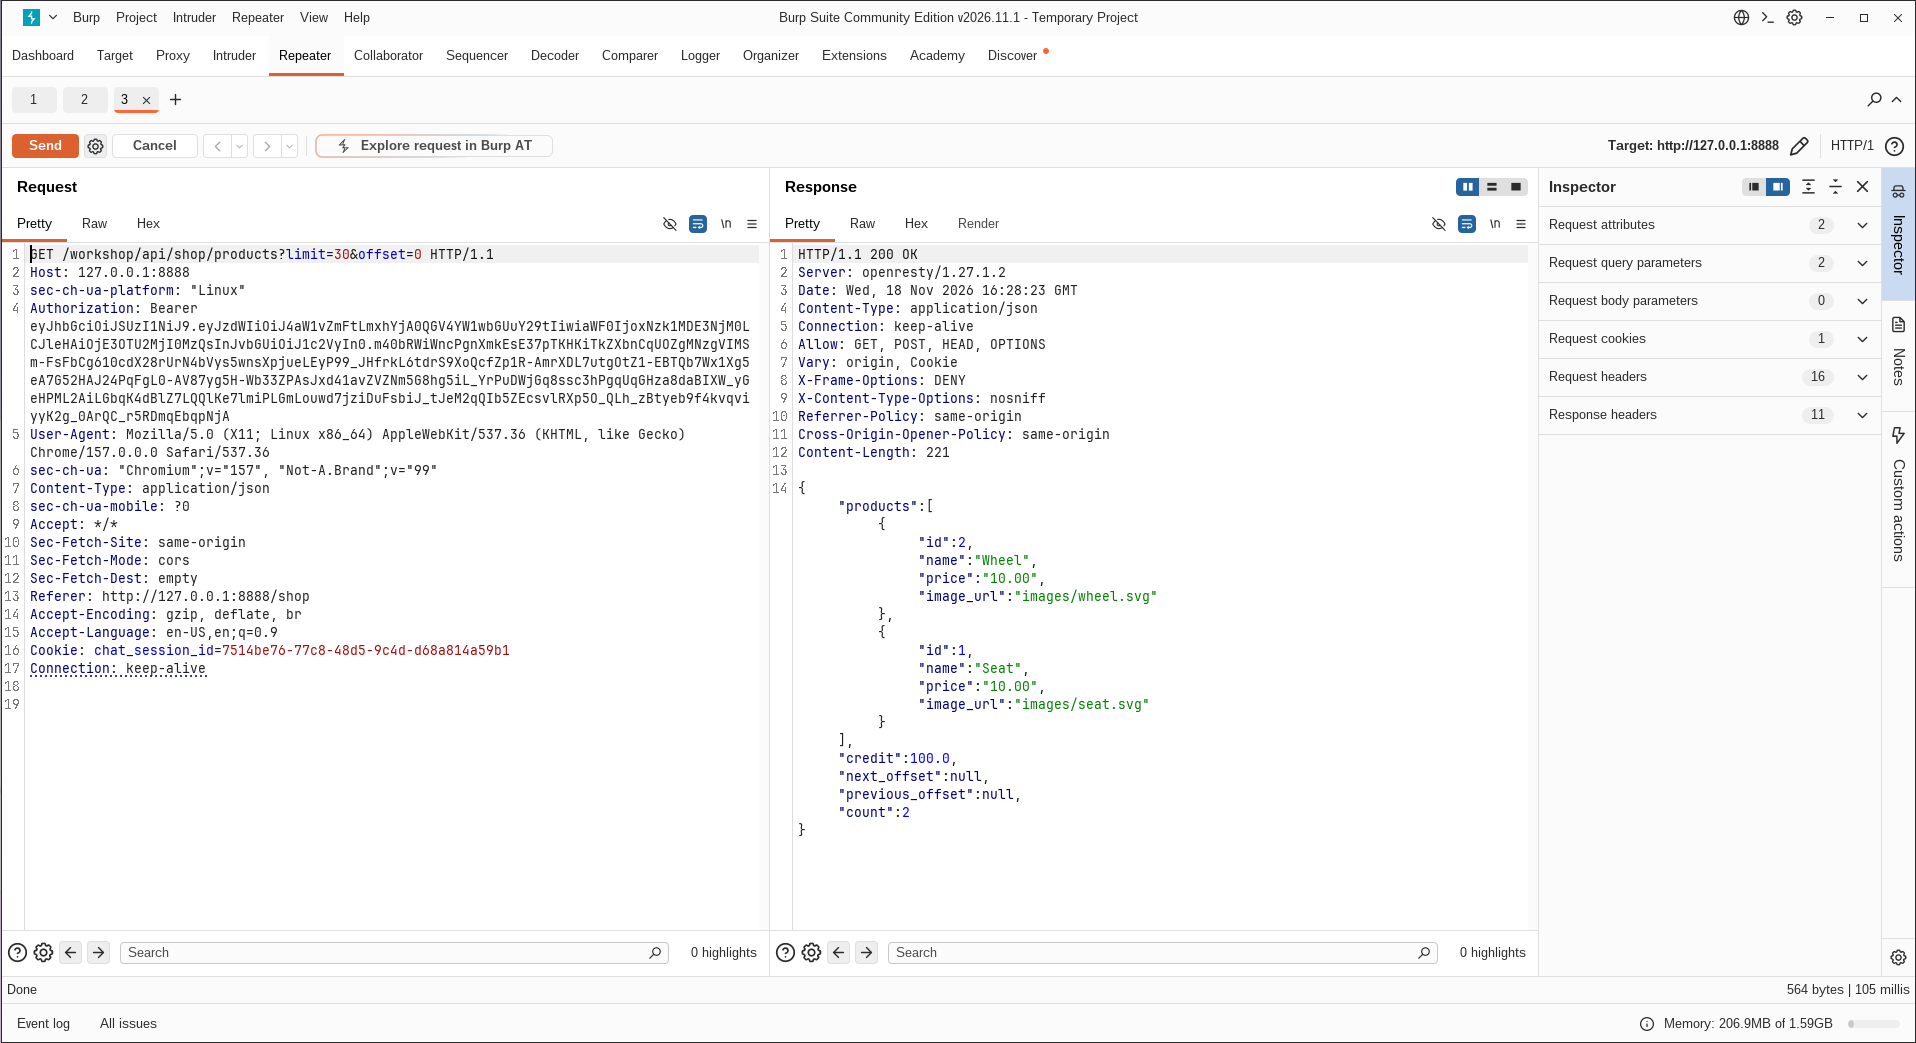
\includegraphics[width=\textwidth,height=0.52\textheight,keepaspectratio]{labs/04-mass-assignment/evidence/09-credit-after-put.png}
    \caption{GET products sau PUT: số dư tăng lên 100.0.}
    \label{fig:mass-credit-after}
\end{figure}

\begin{figure}[htbp]
    \centering
    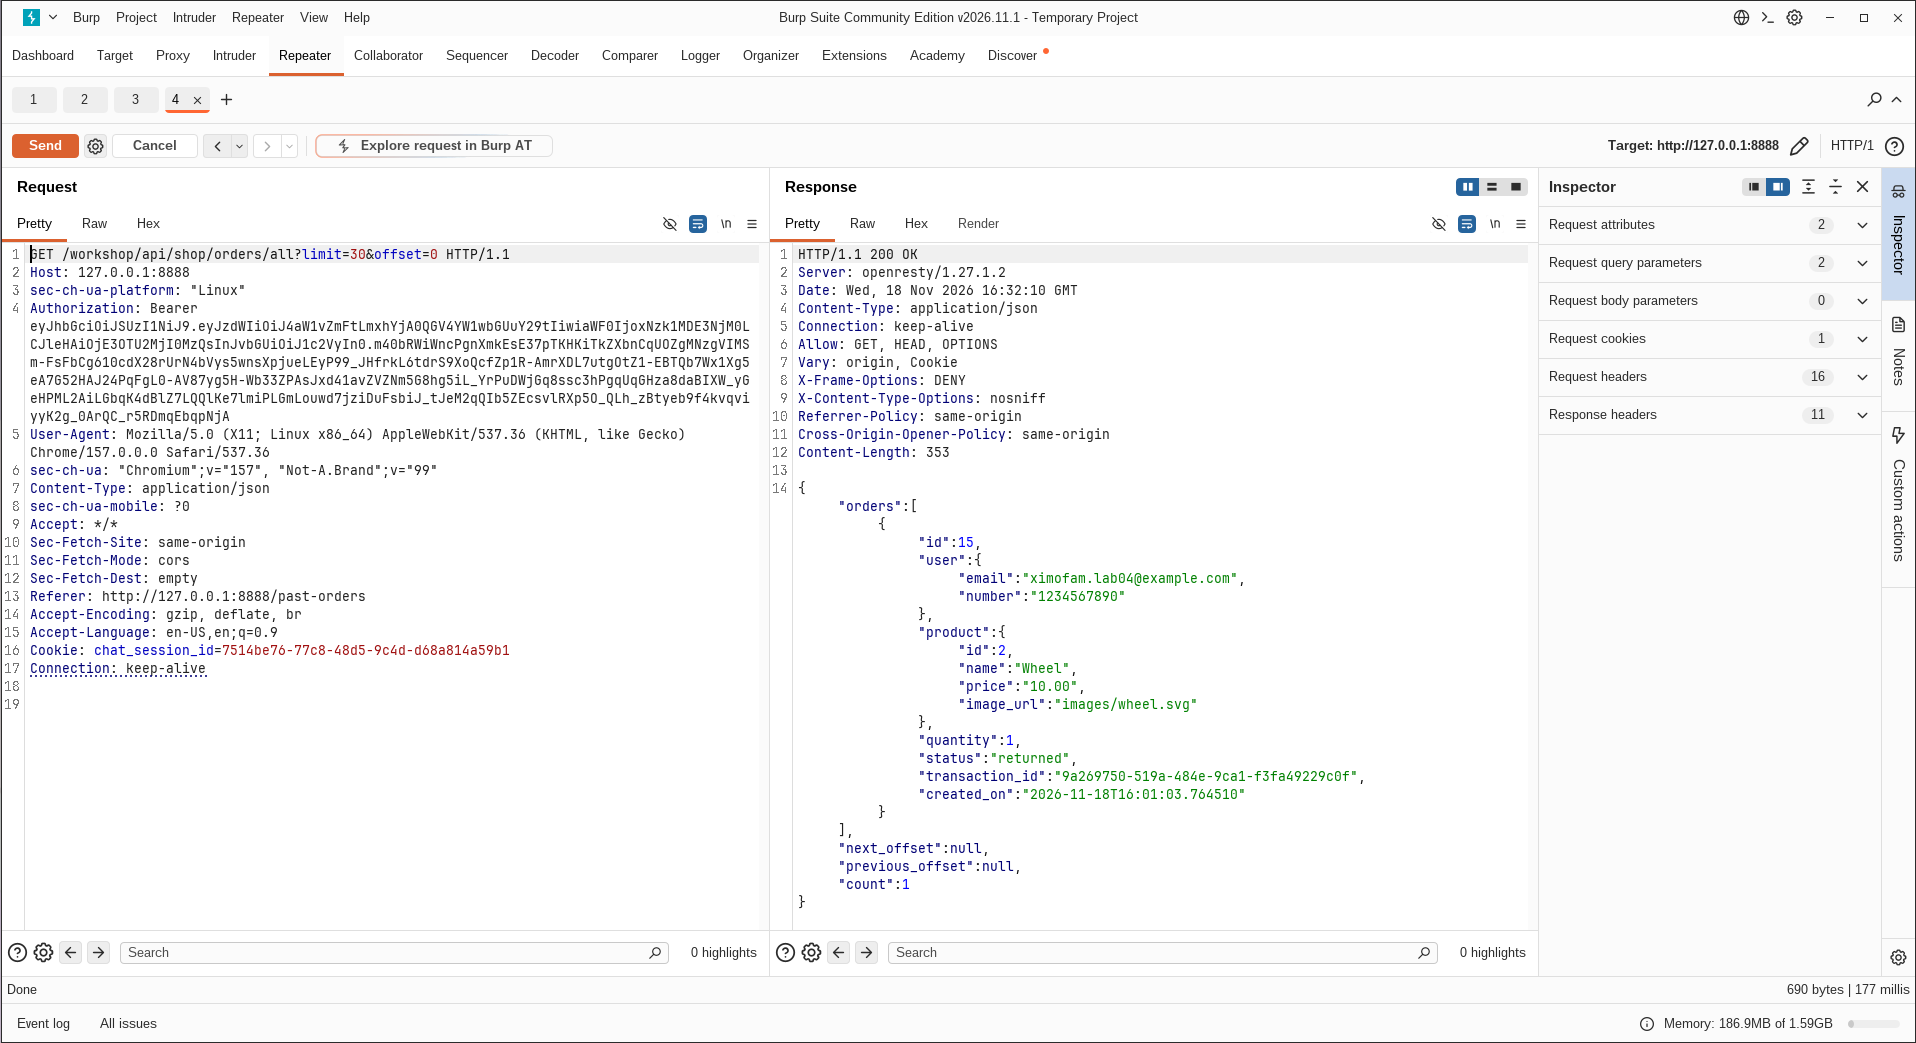
\includegraphics[width=\textwidth,height=0.52\textheight,keepaspectratio]{labs/04-mass-assignment/evidence/10-order-after-put.png}
    \caption{GET orders sau PUT: đơn 15 được lưu với trạng thái returned.}
    \label{fig:mass-order-after}
\end{figure}

Bảng~\ref{tab:mass-assignment-result} tổng hợp kết quả từ ảnh bằng chứng
trước và sau yêu cầu PUT.

\begin{table}[htbp]
    \centering
    \caption{Đối chiếu dữ liệu trước và sau khi sửa trạng thái đơn hàng}
    \label{tab:mass-assignment-result}
    \begin{tabularx}{\textwidth}{@{} X l l @{}}
        \toprule
        \textbf{Dữ liệu} & \textbf{Trước PUT} & \textbf{Sau PUT} \\
        \midrule
        Mã đơn hàng & 15 & 15 \\
        Sản phẩm & Wheel & Wheel \\
        Số lượng & 1 & 1 \\
        Trạng thái & \texttt{delivered} & \texttt{returned} \\
        Số dư & 90.0 & 100.0 \\
        \bottomrule
    \end{tabularx}
\end{table}

Cùng một đơn hàng đã đổi trạng thái và tài khoản được cộng lại
\texttt{10.0}, đúng bằng giá trị đã thanh toán. Hai GET độc lập cho thấy
thay đổi không chỉ nằm trong phản hồi PUT.

Bộ ảnh ghi nhận kết quả này nhưng chưa xác nhận đầy đủ mọi thao tác
xen giữa các mốc. Vì vậy, trước khi kết luận đã bỏ qua toàn bộ quy trình
trả hàng, cần xác nhận người thực hiện không gửi thêm yêu cầu trả hàng
hoặc xác minh khác trong khoảng đó.

\clearpage
\section{Nguyên nhân và tác động}

Trong mã nguồn được đối chiếu, API có kiểm tra đơn hàng thuộc về người
gọi. Tuy nhiên, API vẫn lấy giá trị \texttt{status} từ nội dung yêu cầu
để cập nhật đơn hàng~\cite{crapi-shop}. Việc kiểm tra giá trị có nằm trong danh sách trạng
thái hợp lệ chưa trả lời được câu hỏi: người dùng có quyền thực hiện
chuyển trạng thái đó hay không?

Khi trạng thái được đổi thành \texttt{returned}, máy chủ cộng số lượng
nhân đơn giá vào số dư. Như vậy, một thuộc tính do người dùng cung cấp
lại quyết định việc hoàn tiền mà thiếu bước kiểm soát nghiệp vụ cần thiết.

Trong lần thực nghiệm được ghi nhận, tác động là thay đổi trạng thái
một đơn hàng và tăng số dư từ \texttt{90.0} lên \texttt{100.0}.
Chưa có bằng chứng về hoàn tiền nhiều lần, sửa đơn hàng của người khác
hoặc tác động đến các giao dịch khác.

\section{Kiểm thử tự động}

File \path{tests/security/test_mass_assignment.py} có bài kiểm thử tạo
một đơn hàng thử, gửi yêu cầu đổi trạng thái rồi dùng hai GET để đọc lại
trạng thái và số dư. Yêu cầu bảo mật là thao tác này không được tự đổi
trạng thái trả hàng hoặc làm tăng số dư.

Bài kiểm thử trực tiếp chỉ chạy khi chủ động đặt
\path{CRAPI_LAB04_RUN=1} và cấu hình tài khoản thử nghiệm. Nó tạo một
đơn hàng có thanh toán và không tự khôi phục dữ liệu. Khi bật chạy trực
tiếp, lệnh kiểm thử là:

\begin{Verbatim}[breaklines=true,breakanywhere=true,fontsize=\small]
CRAPI_LAB04_RUN=1 pytest tests/security/test_mass_assignment.py -m security -v
\end{Verbatim}

Khi kiểm tra bộ test ở chế độ không gọi crAPI thật, kết quả là
\texttt{6 passed, 1 skipped}. Sáu bài kiểm tra mô phỏng xác nhận logic
test phân biệt được tình huống bị từ chối và tình huống đổi trạng thái
hoặc tăng tiền trái phép. Bài gọi crAPI thật bị bỏ qua; kết quả này
không thay thế bằng chứng khai thác thủ công và không chứng minh hệ
thống đã được vá.

\section{Biện pháp khắc phục và kết luận}

Các biện pháp khắc phục được đề xuất gồm:
\begin{enumerate}
    \item Chỉ nhận những thuộc tính người dùng được phép sửa. Không cho
    cập nhật trực tiếp trạng thái hoàn trả hoặc dữ liệu thanh toán qua
    API sửa đơn hàng thông thường.
    \item Kiểm soát trình tự chuyển trạng thái ở máy chủ. Chỉ chuyển
    sang đã trả hàng sau khi bên có thẩm quyền xác nhận đủ điều kiện.
    \item Tính tiền hoàn từ giao dịch gốc, không vượt quá số đã thanh
    toán. Mỗi lần hoàn cần có mã giao dịch riêng và được xử lý nhất quán
    để tránh cộng tiền nhiều lần.
\end{enumerate}

Sau khi sửa, yêu cầu PUT trực tiếp phải bị từ chối hoặc không làm thay
đổi trạng thái và số dư; quy trình trả hàng hợp lệ vẫn phải hoạt động.
Hiện chưa có bản vá hoặc kết quả kiểm thử sau vá trong hồ sơ Lab.

Kết quả ghi nhận cho thấy API chấp nhận trạng thái do người dùng gửi,
lưu trạng thái \texttt{returned} và cộng lại tiền cho đơn hàng thử.
Điểm cần bảo vệ không chỉ là quyền sở hữu đơn hàng mà còn là quyền
thay đổi từng thuộc tính có ảnh hưởng đến nghiệp vụ hoàn tiền.



\clearpage
\chapter{Lab 05: Đọc đơn hàng khi chưa xác thực (Unauthenticated Access)}
\label{chap:lab05}

\section{Bài toán và mục tiêu kiểm thử}

Chi tiết đơn hàng chứa sản phẩm, thông tin người mua và giao dịch.
Đây là dữ liệu cần bảo vệ: máy chủ phải xác minh người gọi trước khi
trả dữ liệu, rồi kiểm tra người đó có quyền xem đơn hàng hay không.

Lab này kiểm tra bước xác thực. Một yêu cầu không có token hoặc có
token sai phải bị từ chối, thay vì vẫn đọc được đơn hàng. Đây là tình
huống thiếu kiểm tra xác thực, liên quan đến nhóm Broken
Authentication của OWASP~\cite{owasp-authentication}.

\section{Chuẩn bị và hành vi mong đợi}

Trên crAPI cục bộ tại \url{http://127.0.0.1:8888}, tạo tài khoản thử
nghiệm và mua một sản phẩm để có đơn hàng hợp lệ. Khi mở Order Details
trên giao diện, trình duyệt gửi token đăng nhập kèm yêu cầu lấy chi tiết.
Đơn hàng dùng trong bản ghi thủ công có mã 6.


\begin{figure}[htbp]
    \centering
    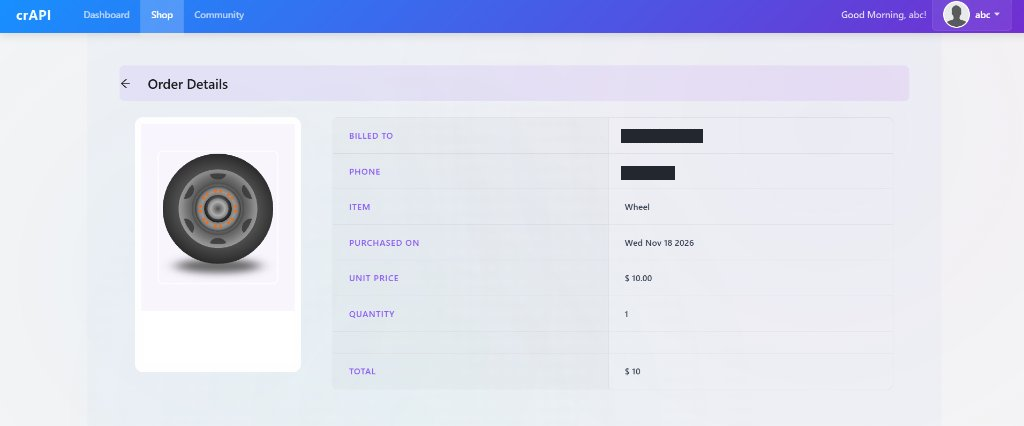
\includegraphics[width=\textwidth,height=0.65\textheight,keepaspectratio]{labs/05-unauthenticated-access/evidence/01-shop-order-details-ui.png}
    \caption{Giao diện chi tiết đơn hàng trong phiên đăng nhập hợp lệ.}
    \label{fig:lab5-ui}
\end{figure}


Hai API được dùng để đối chiếu:
\begin{Verbatim}[breaklines=true,breakanywhere=true,fontsize=\small]
GET /workshop/api/shop/orders/all
GET /workshop/api/shop/orders/{order_id}
\end{Verbatim}

API thứ nhất trả danh sách đơn hàng, API thứ hai trả chi tiết một đơn.
Cả hai cần từ chối bằng \texttt{401 Unauthorized} khi không có thông
tin xác thực hợp lệ.

\section{Các bước kiểm thử và bằng chứng}

\subsection{Kiểm tra API đối chứng}

Gửi yêu cầu lấy danh sách đơn hàng mà không có token:
\begin{Verbatim}[breaklines=true,breakanywhere=true,fontsize=\small]
GET /workshop/api/shop/orders/all HTTP/1.1
Host: 127.0.0.1:8888
\end{Verbatim}

API trả \texttt{401} với thông báo \texttt{JWT Token required!}.
Kết quả cho thấy dịch vụ có cơ chế kiểm tra token đang hoạt động ở API
đối chứng; không phải mọi API của dịch vụ đều bỏ qua xác thực.

\subsection{Bỏ token khi lấy chi tiết đơn hàng}

Gửi yêu cầu sau mà không có header Authorization và không có cookie:
\begin{Verbatim}[breaklines=true,breakanywhere=true,fontsize=\small]
GET /workshop/api/shop/orders/6 HTTP/1.1
Host: 127.0.0.1:8888
\end{Verbatim}

Máy chủ vẫn trả \texttt{HTTP 200} cùng dữ liệu đơn hàng. Phản hồi đã
lưu có mã đơn, sản phẩm, số lượng, trạng thái, thông tin người mua và
thông tin thanh toán. Số thẻ trong dữ liệu thanh toán đã được che một
phần; không kết luận toàn bộ số thẻ bị lộ.


\begin{figure}[htbp]
    \centering
    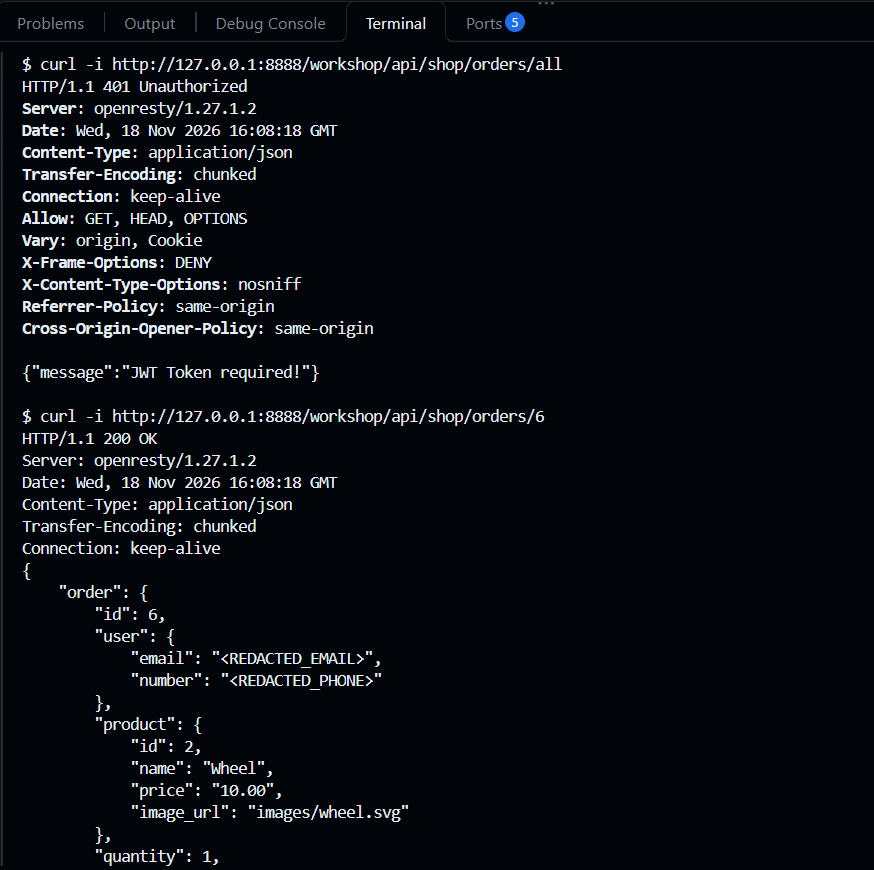
\includegraphics[width=\textwidth,height=0.65\textheight,keepaspectratio]{labs/05-unauthenticated-access/evidence/02-curl-unauthenticated-access.png}
    \caption{Cùng không có token: danh sách đơn hàng trả 401, chi tiết đơn hàng trả 200.}
    \label{fig:lab5-curl}
\end{figure}


\subsection{Thay token bằng giá trị không hợp lệ}

Gửi lại yêu cầu với token sai:
\begin{Verbatim}[breaklines=true,breakanywhere=true,fontsize=\small]
GET /workshop/api/shop/orders/6 HTTP/1.1
Host: 127.0.0.1:8888
Authorization: Bearer invalid.jwt.token
\end{Verbatim}

Bản ghi HTTP và kết quả test đều ghi nhận API vẫn trả \texttt{200}.
Như vậy, vấn đề không chỉ là chấp nhận yêu cầu thiếu token: API cũng
không từ chối token không hợp lệ.

\begin{table}[htbp]
\centering
\caption{Kết quả kiểm tra xác thực trên hai API đơn hàng}
\label{tab:unauthenticated-result}
\begin{tabularx}{\textwidth}{@{} X l l @{}}
\toprule
\textbf{Yêu cầu} & \textbf{Kỳ vọng} & \textbf{Thực tế} \\
\midrule
Danh sách đơn hàng, không token & 401 & 401 \\
Chi tiết đơn hàng, không token & 401 & 200 \\
Chi tiết đơn hàng, token sai & 401 & 200 \\
\bottomrule
\end{tabularx}
\end{table}

\clearpage
\section{Nguyên nhân và tác động}

Đối chiếu mã nguồn xử lý Shop~\cite{crapi-shop} cho thấy phương thức
lấy chi tiết đơn hàng không có bước kiểm tra JWT, trong khi phương
thức tạo, cập nhật và lấy danh sách đơn hàng có kiểm tra này. Cấu hình
framework cũng chưa đặt yêu cầu đăng nhập mặc định cho mọi API được
bảo vệ. Vì vậy, phương thức bị bỏ sót vẫn có thể xử lý yêu cầu.

Giao diện luôn tự gửi token có thể khiến lỗi khó nhận ra nếu chỉ kiểm
tra thao tác thông thường. Khi gửi yêu cầu trực tiếp bằng curl hoặc
HTTP client, việc thiếu kiểm tra ở máy chủ mới thể hiện rõ.

Tác động đã ghi nhận là đọc được dữ liệu của đơn hàng thử khi chưa
xác thực. Lab chưa chứng minh người không đăng nhập có thể tạo, sửa
hoặc xóa đơn hàng. Việc sửa trạng thái đơn hàng trong Lab 04 là một
kịch bản khác, sử dụng tài khoản đã đăng nhập.

\section{Kiểm thử tự động}

File \path{tests/security/test_unauthenticated_access.py} có ba test:
kiểm tra API đối chứng, kiểm tra thiếu token và kiểm tra token sai.
Bộ test tự tạo tài khoản cùng đơn hàng thử, nên làm thay đổi dữ liệu
Lab. Chạy bằng:
\begin{Verbatim}[breaklines=true,breakanywhere=true,fontsize=\small]
pytest tests/security/test_unauthenticated_access.py -v --tb=short
\end{Verbatim}

Ảnh kết quả thực nghiệm ghi nhận:
\begin{Verbatim}[breaklines=true,breakanywhere=true,fontsize=\small]
2 failed, 1 passed in 2.63s
\end{Verbatim}

Test đối chứng PASSED vì API danh sách trả đúng \texttt{401}. Hai test
chi tiết FAILED vì nhận \texttt{200} thay cho \texttt{401}, phù hợp
với bằng chứng thiếu xác thực. Mã đơn 10 và 11 trong ảnh test khác mã
6 ở phần thủ công vì test tự tạo đơn hàng riêng.


\begin{figure}[htbp]
    \centering
    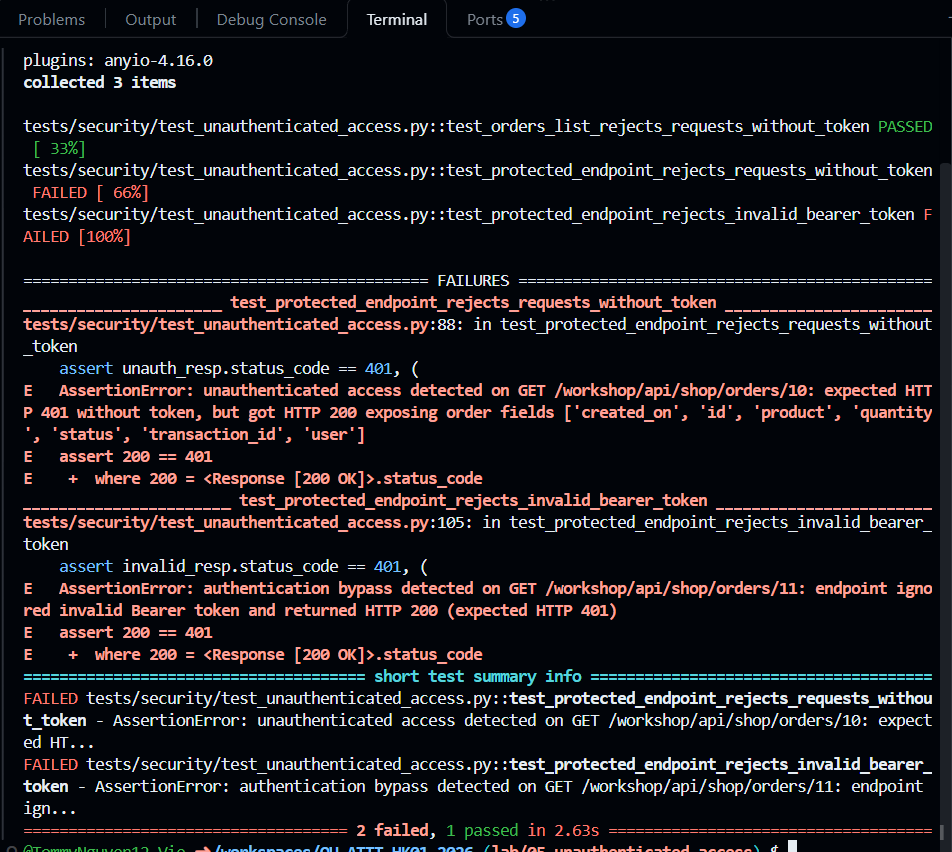
\includegraphics[width=\textwidth,height=0.65\textheight,keepaspectratio]{labs/05-unauthenticated-access/evidence/03-pytest-security-result.png}
    \caption{Kết quả pytest: một test đối chứng PASS, hai test xác thực chi tiết đơn hàng FAIL.}
    \label{fig:lab5-pytest}
\end{figure}


\clearpage
\section{Biện pháp khắc phục và kết luận}

Các biện pháp đề xuất gồm:
\begin{enumerate}
    \item Bổ sung kiểm tra JWT cho phương thức lấy chi tiết đơn hàng;
    trả \texttt{401} khi thiếu token, token sai hoặc hết hạn.
    \item Cấu hình mặc định yêu cầu xác thực cho API cần bảo vệ và chỉ
    cho phép truy cập tự do ở những chức năng công khai được chỉ định.
    \item Sau khi xác thực, tiếp tục kiểm tra quyền sở hữu đơn hàng
    trước khi trả dữ liệu; đăng nhập hợp lệ chưa đủ để xem mọi đơn.
    \item Chạy lại ba test và xác nhận yêu cầu hợp lệ vẫn nhận đúng dữ
    liệu, còn yêu cầu thiếu hoặc sai token đều bị từ chối. Kiểm tra
    tương tự cho từng HTTP method để tránh bỏ sót.
\end{enumerate}

Lab ghi nhận chi tiết đơn hàng vẫn được trả về khi không có token
hoặc token không hợp lệ. Kết quả thủ công và ảnh pytest cùng xác nhận
bước kiểm tra xác thực bị thiếu ở API này. Chưa có bản vá hoặc kết quả
kiểm thử sau vá trong bộ bằng chứng.

\clearpage
\begin{thebibliography}{9}
    \bibitem{crapi}
    OWASP, \textit{crAPI --- Completely Ridiculous API}.
    Mã nguồn và tài liệu giới thiệu hệ thống.
    \url{https://github.com/OWASP/crAPI}.

    \bibitem{owasp-bola}
    OWASP, \textit{API1:2023 --- Broken Object Level Authorization},
    OWASP API Security Top 10, 2023.
    \url{https://owasp.org/API-Security/editions/2023/en/0xa1-broken-object-level-authorization/}.

    \bibitem{crapi-vehicle}
    OWASP crAPI, \textit{VehicleServiceImpl.java}.
    Mã nguồn xử lý dữ liệu phương tiện, dùng để đối chiếu nguyên nhân BOLA.
    \url{https://github.com/OWASP/crAPI/blob/main/services/identity/src/main/java/com/crapi/service/Impl/VehicleServiceImpl.java}.

    \bibitem{owasp-bfla}
    OWASP, \textit{API5:2023 --- Broken Function Level Authorization},
    OWASP API Security Top 10, 2023.
    \url{https://owasp.org/API-Security/editions/2023/en/0xa5-broken-function-level-authorization/}.

    \bibitem{owasp-exposure}
    OWASP, \textit{API3:2019 --- Excessive Data Exposure},
    OWASP API Security Top 10, 2019.
    \url{https://owasp.org/API-Security/editions/2019/en/0xa3-excessive-data-exposure/}.

    \bibitem{owasp-property}
    OWASP, \textit{API3:2023 --- Broken Object Property Level Authorization},
    OWASP API Security Top 10, 2023.
    \url{https://owasp.org/API-Security/editions/2023/en/0xa3-broken-object-property-level-authorization/}.

    \bibitem{crapi-shop}
    OWASP crAPI, \textit{Shop views.py}.
    Mã nguồn cập nhật đơn hàng và xử lý yêu cầu trả hàng.
    \url{https://github.com/OWASP/crAPI/blob/main/services/workshop/crapi/shop/views.py}.
    \bibitem{owasp-authentication}
    OWASP, \textit{API2:2023 --- Broken Authentication},
    OWASP API Security Top 10, 2023.
    \url{https://owasp.org/API-Security/editions/2023/en/0xa2-broken-authentication/}.
\end{thebibliography}

\end{document}
